\documentclass{article}

\title{Take Me Out to (Analyze) the Ballgame}
\author{Chris Comiskey}
\date{\today}

\usepackage{natbib}
\bibliographystyle{unsrtnat}

\usepackage{fullpage}
\usepackage{ulem}
\usepackage{amsmath, amsthm, amssymb, amsfonts}
\usepackage{mathtools}
\usepackage{float}
\usepackage{bbm}
\usepackage{wrapfig}
\usepackage{listings}
\usepackage[utf8]{inputenc}
\usepackage[english]{babel}
\usepackage[export]{adjustbox}

\makeatletter
\def\verbatim@font{\linespread{1}\normalfont\ttfamily}
\makeatother

\usepackage[toc,page]{appendix}


% \setlength{\parindent}{4em}
% \setlength{\parskip}{1em}
% \renewcommand{\baselinestretch}{1.3}

\usepackage{setspace}
\doublespacing

\begin{document}
\maketitle{}

\tableofcontents


\section{Introduction}
Graphical displays are an irreplaceable tool for the statistician, and the statistical community. They allow us to quickly communicate information about a data set to another statistician, or, perhaps even more importantly, to non-statisticians. As technology generates more data the importance of this area of statistics expands, statistical analysis becomes more widespread, and our graphic-making abilities improve. The R data visualization package \verb|ggplot2| highlights (i) the importance of graphical diplays, because it is among the most downloaded R packages; and (ii) the need for innovation in this area, because its popularity explosion signals it met a need.

In this chapter we focus on one type of graphical display, the heat map. We show the way it fails to adequately communicate spatial data dispersion and distribution attributes, and we innovate a solution. This innovation improves our ability to communicate spatial data density and dispersion attributes to the viewer using a heat map.

\section{Heat Maps} % ==================== 


\subsection{Conventional Heat Maps} % ==================== 

We start with a baseball heat map example, as baseball data motivates this research. Consider the empirical heat map in Figure 1, of the two dimensioned vertical face of the strike zone, where grid box colors represent empirical batting averages at pitch locations. In Figure 1 we show PITCHf/x\textsuperscript{\textregistered} data on 1,932 right-handed hitters, taking 1,582,581 swings between 2008 and 2015.  Let $b = 1, \dots, 627$ index grid boxes. Let $i = 1, \dots, 1,582,581$ index swings, and define $n_{b} = \displaystyle\sum_{i} \text{I}_{\{i \in b \}}$ as the total number of swings in box $b$.
Define a Bernoulli random variable, $S_{i}$, that equals one for swing success and zero for swing failure, and let $\hat{p}_{b} = \frac{1}{n_{b}} \displaystyle\sum_{i} S_{i} \cdot \text{I}_{\{i \in b \}}$ be the empirical box $b$ success probability. Figure 1 displays the resulting empirical heat map for 1,932 right-handed hitters, taking 1,582,581 swings between 2008 and 2015. The heat map graphic maps the empirical success probability, $\hat{p}_{b}$, of hitters swinging at pitches that passed through the space represented by that grid box, to a color on a spectrum.
  \begin{figure}[H]
	\centering
	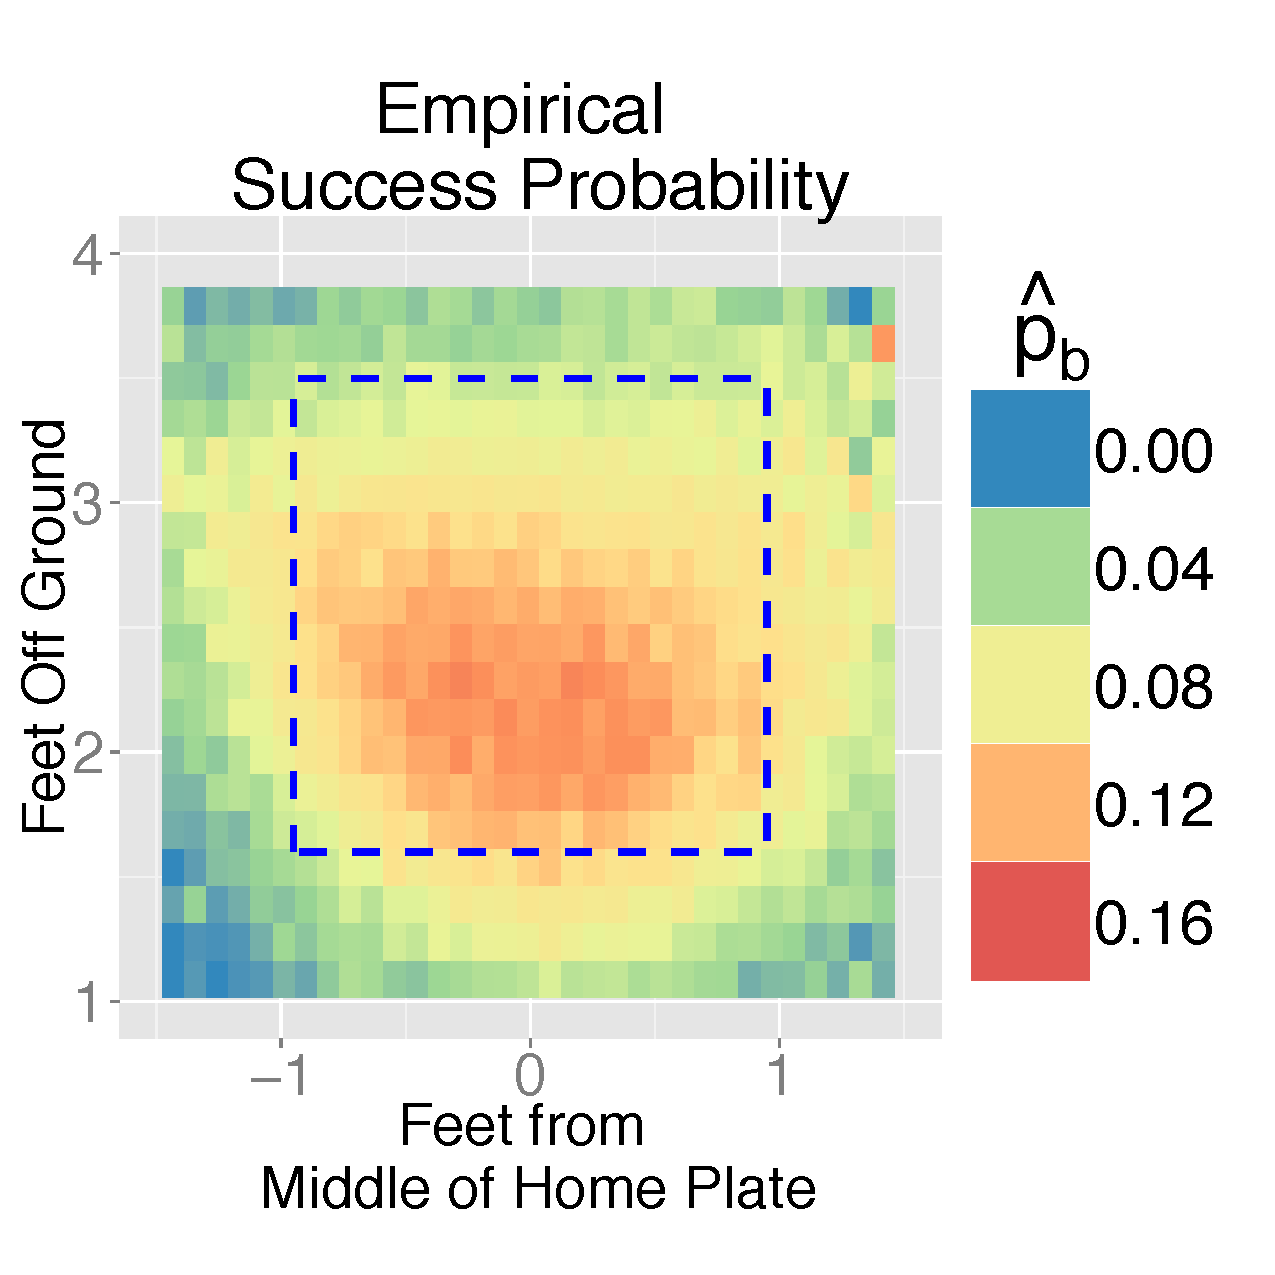
\includegraphics[scale=.3]{Images/Mothership.pdf} 
  \caption{The gridded hitting zone with 3/4 inch by 3/4 inch boxes, from the catcher's point of view. The color of the box represents the empirical batting average ($\hat{p}_{b}$) for right handed hitters, swinging at pitches in that location. Calculations based on 1,932 right handed hitters, swinging at 1,582,581 pitches between 2008 and 2015. The dashed line marks the boundaries of the called strike zone for a 6'2'' hitter.}
	\end{figure} 
\noindent While not sophisticated statistically, the graphic efficiently conveys empirical spatial success probabilities; it maps the statistic $\hat{p}_{b}$ to a color on a spectrum. Though it can easily go unnoticed, a heat map's creater {\it chooses} the grid box size that, hopefully, best communicates the data's information content; here, average spatial hitting ability estimates. The data's varying spatial density through the strike zone is not part of the communicated information, no matter the grid box size selected. This missing information is important, because in general more data means better estimates, and the viewer gets no such indication in Figure 1. Traditional heat maps do not communicate this information. We propose an innovation that addresses this shortcoming. To illustrate, consider a heat map for an individual hitter.

The heat map above divided the strike zone into relatively small boxes, because the data supported it. By ``supported it'' we mean the small, spatially specific boxes retain a sample size large enough to keep the variance of $\hat{p}_{b}$ acceptably \footnote{Defining ``acceptable'' variance ranges and thresholds will depend on context and analysis objectives. For example, a pitching coach may be satisfied with estimates accurate 95\% of the time to within 20 batting average points. This margin of error, 0.02, requires a sample size of 32 when $p_{b} = 0.09$. Note that the variance depends on the mean for a Bernoulli random variable.} This is important because individual hitter datasets vary dramatically in size, with swing totals ranging from a single swing to over 10,000 swings. Similar to bin width selection for a histogram, the choice of heat map resolution can dramatically affect how the data is represented, and the usefulness of the parameter estimates of interest. The resolution decision depends on the size and nature of the data set in question, and its spatial dispersion through the domain. To explore this decision in detail we look at batter 425509, a veteran player named Jhonny Peralta, whose data set contains 9,177 swings.

\subsection{Empirical Heat Maps and Resolution Selection} % ==============

The heat map in Figure 2 divides the central region of the strike zone into 16 equally sized boxes. Each box maps $\hat{p}_{b}$ to a color, and the box sample size, $n_{b}$, is printed on the box center. For convenient referencing in this chapter, we adopt the convention of numbering boxes with a horizontal component (left to right) and a vertical component (bottom to top [ {\bf Alix: ``WHY?''}]). For example, we call the top-left box (1,4), and the bottom-right box (4,1). 
        \begin{figure}[H]
      	\centering
      	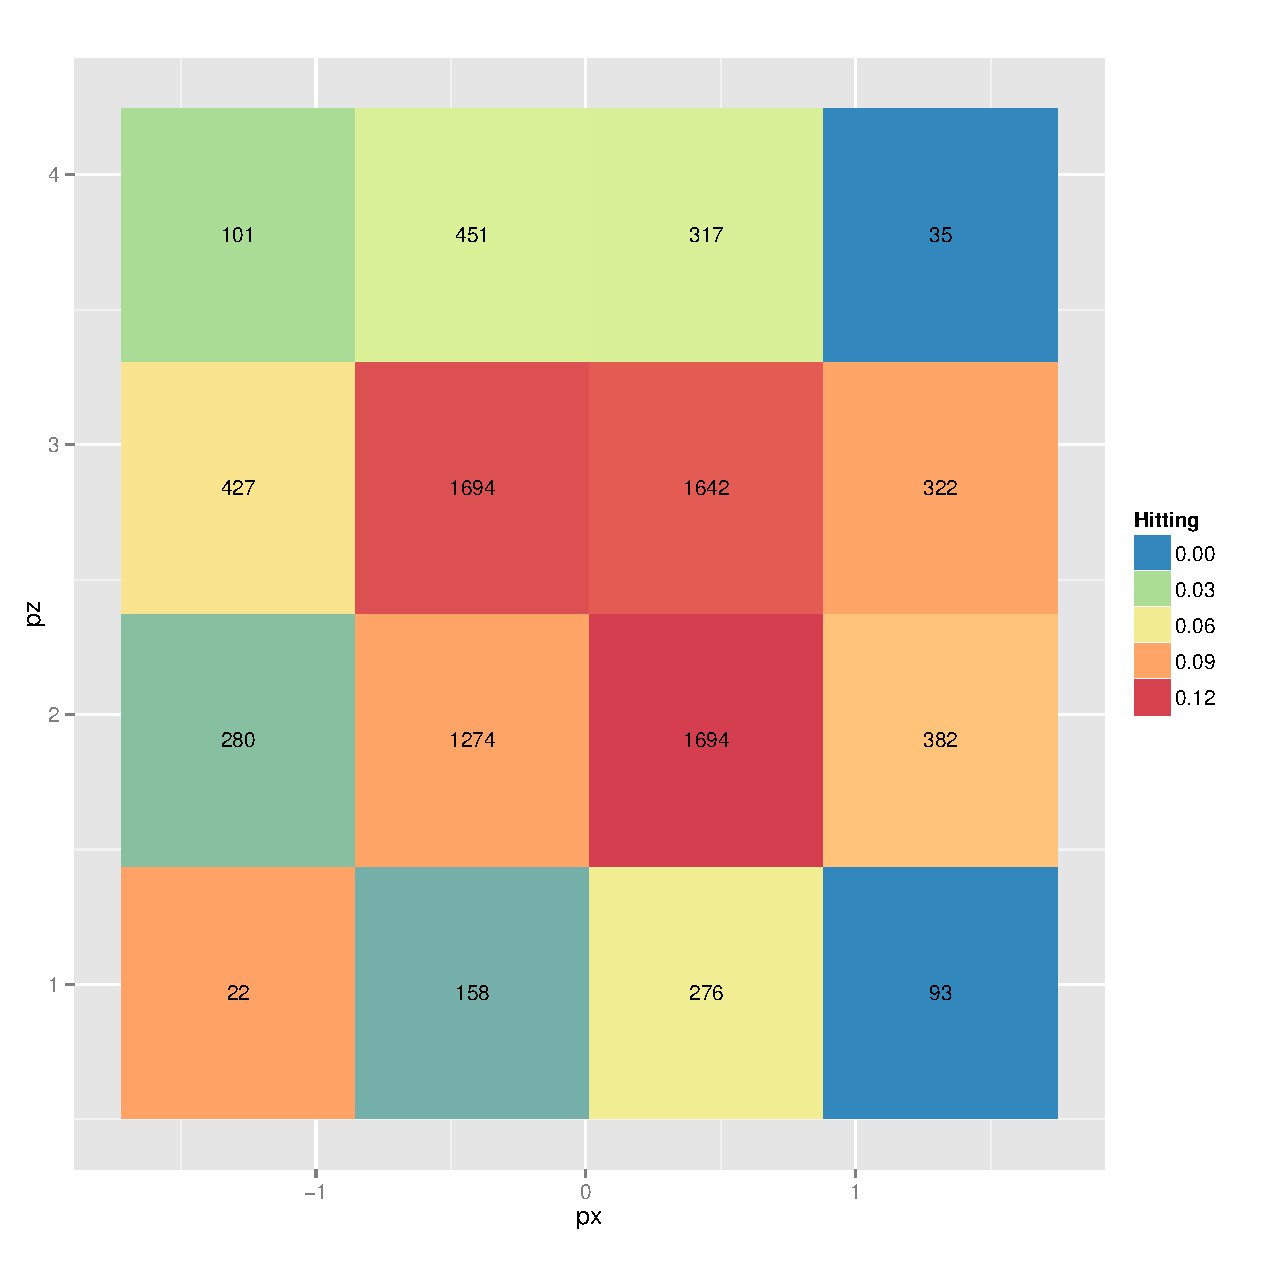
\includegraphics[scale=.35]{Images/Chapter4x4.pdf} 
      	\caption{This four by four heat map conveys the empirical batting average of batter 425509, Johnny Peralta, in each of 16 square regions of the hitting zone. Each box maps $\hat{p}_{b}$ to a color. The number printed on each box represents the number of pitches the hitter swung at that passed through that box.}
      	\end{figure} 

Peralta swang at 22 pitches in the region of space represented by box (1,1), and he swung at 1694 pitches in box (2,3). We interpret these two box sample sizes to contextualize. Three primary factors influence pitch location: pitcher game theoretic strategy, pitch-swing location margin of error (distance by which a pitch misses its intended target), and the game state. Game theoretic strategy concerns the pitcher's knowledge of the hitter's strenths and weaknesses, and the hitter's reciprocal knowledge. Margin of error concerns the pitcher's usual outcome of not exactly hitting his target.\footnote{If you visualize a 12 inch diameter archery target where the pitcher aims, he will usually hit the target somewhere, but not the bull's-eye.} Game state characteristics include the at-bat count, the number of outs, and if runners occupy bases.\footnote{Two example game state pressures include the increased penalty for throwing a pitch outside the strike zone on a three ball count (the runner gets on base at four balls); the increased penalty for a hit with a runner in scoring position (runner on second or third base).} Peralta probably swung at only 22 pitches in box (1,1) because he did not see many pitches there. We can speculate this is because pitches there are mostly out of the strike zone, both in the horizontal and vertical directions. Therefore, it is less likely to induce a swing at a bad pitch to hit, and unlikely to be called a strike despite being out of the strike zone. With $n_{(1,1)}=22$, the four by four resolution is sufficiently fine to present $\hat{p}_{(1,1)}$. Box (2,3), with $n_{(2,3)} = 1694$ pitches, can support more location specific, but still reliable estimates of $p$. This motivates finer resolution in that region of space. Peralta has relatively high success in Box (2,3), and he undoubtedly swings at as many pitches in that box as possible. The pitcher knows this, so will seldom aim there. However, by virtue of being closer to the center of the strike zone, this location collects more pitch location mistakes.

Because, as mentioned, a finer resolution is justified for box (2,3), we subdivide all boxes further. For simplicity, without implying this is the only or best way to increase resolution, we divide each box into four equally sized sub-boxes. Figure 3 shows the 16 by 16 result.
        \begin{figure}[H]
      	\centering
      	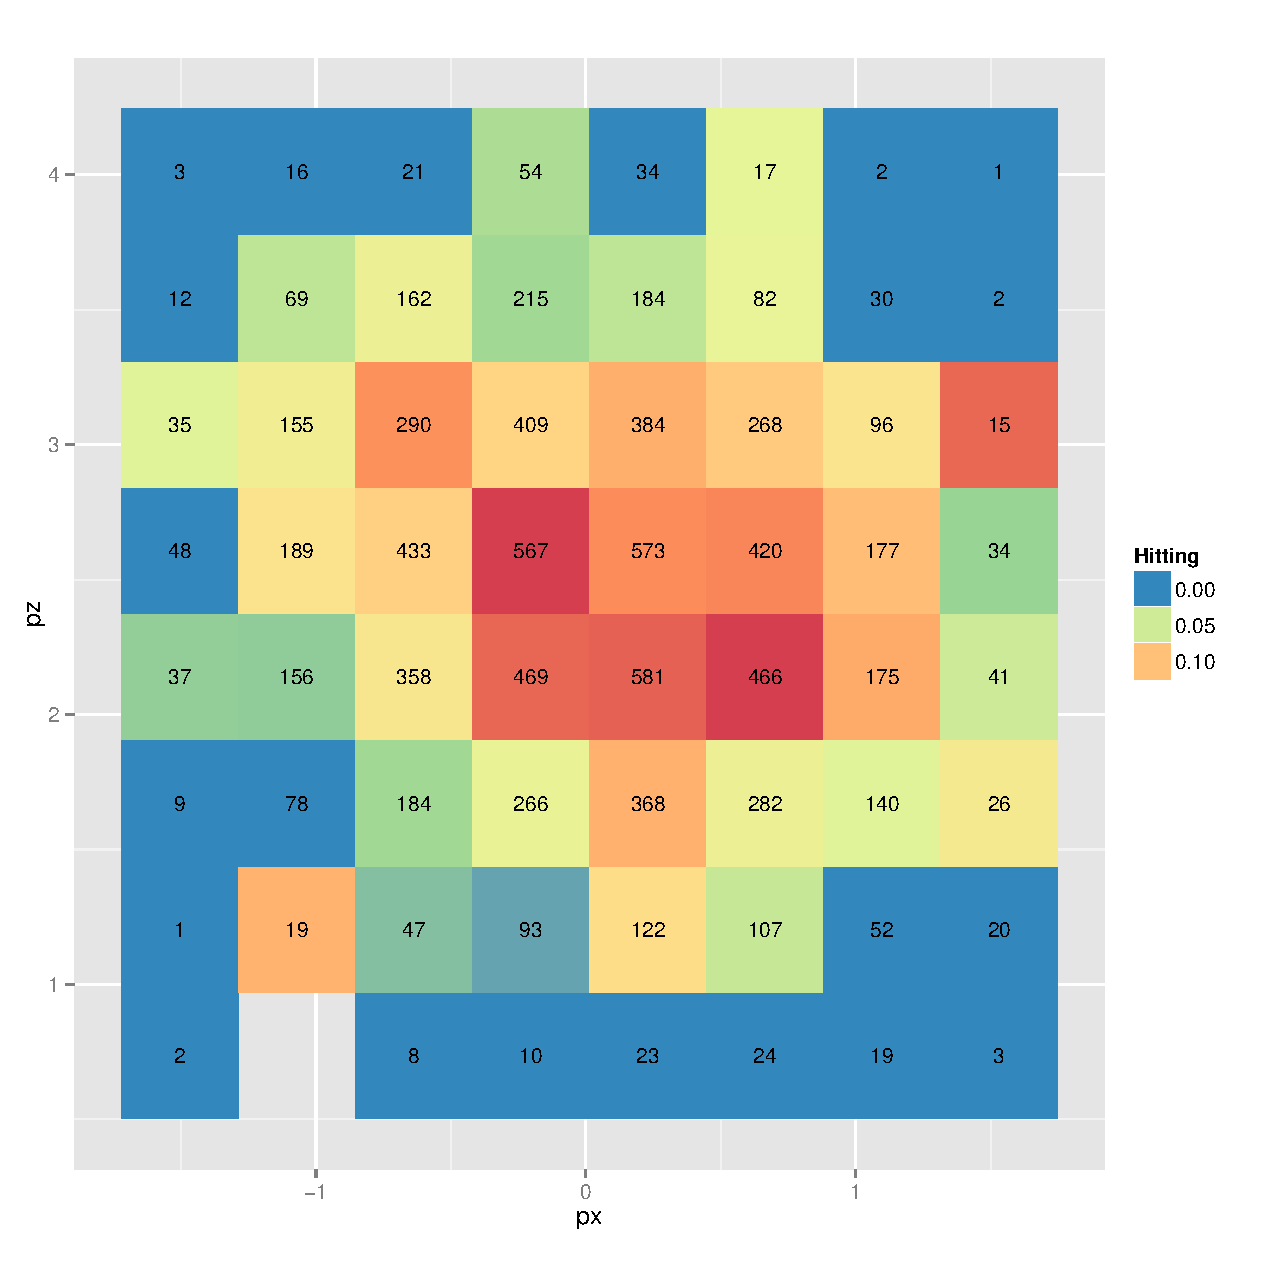
\includegraphics[scale=.25]{Images/Chapter16x16.pdf} 
      	\caption{This 16 by 16 heat map conveys the empirical batting average of batter 425509, Johnny Peralta, in each of 64 square regions of the hitting zone. Each box maps $\hat{p}_{b}$ to a color. The number printed on each box gives the number of pitches the hitter swung at that passed through that box. A grey box indicates no pitches passed through that box.}
      	\end{figure} 

Boxes (3,5), (3,6), (4,5), and (4,6)---the boxes created by dividing box (2,3) at the four by four resolution---still contain sample sizes sufficient to support low variance $p$ estimates. More generally, 24 boxes still have a sample size greater than 150; and 15 boxes still have a sample size of greater than 250. These boxes could support further subdivision. On the other hand, numerous boxes---corner and edge boxes in particular---now contain sample sizes generally insufficient to support low variance estimates of $p_{b}$. Twenty-nine boxes have a sample size of less than 50, and 17 boxes have a sample size of less than 20. At this resolution one box recorded zero swings.

In this way, due to the particular dispersion of the data, a heat map at any resolution will contain boxes of exceedingly small sample sizes (high variance), and/or boxes of unnecessarily large sample size (unnecessarily low variance). Figure 3 shows six different heat map resolutions, constructed with the same data from Peralta. We started with one box, and subdivided each box into four at each iteration. We chose this simple resolution increasing algorithm to illustrate the resolution selection challenge, and to provide a foundation for our innovation in the next section. 
        \begin{figure}[H]
      	\centering
      	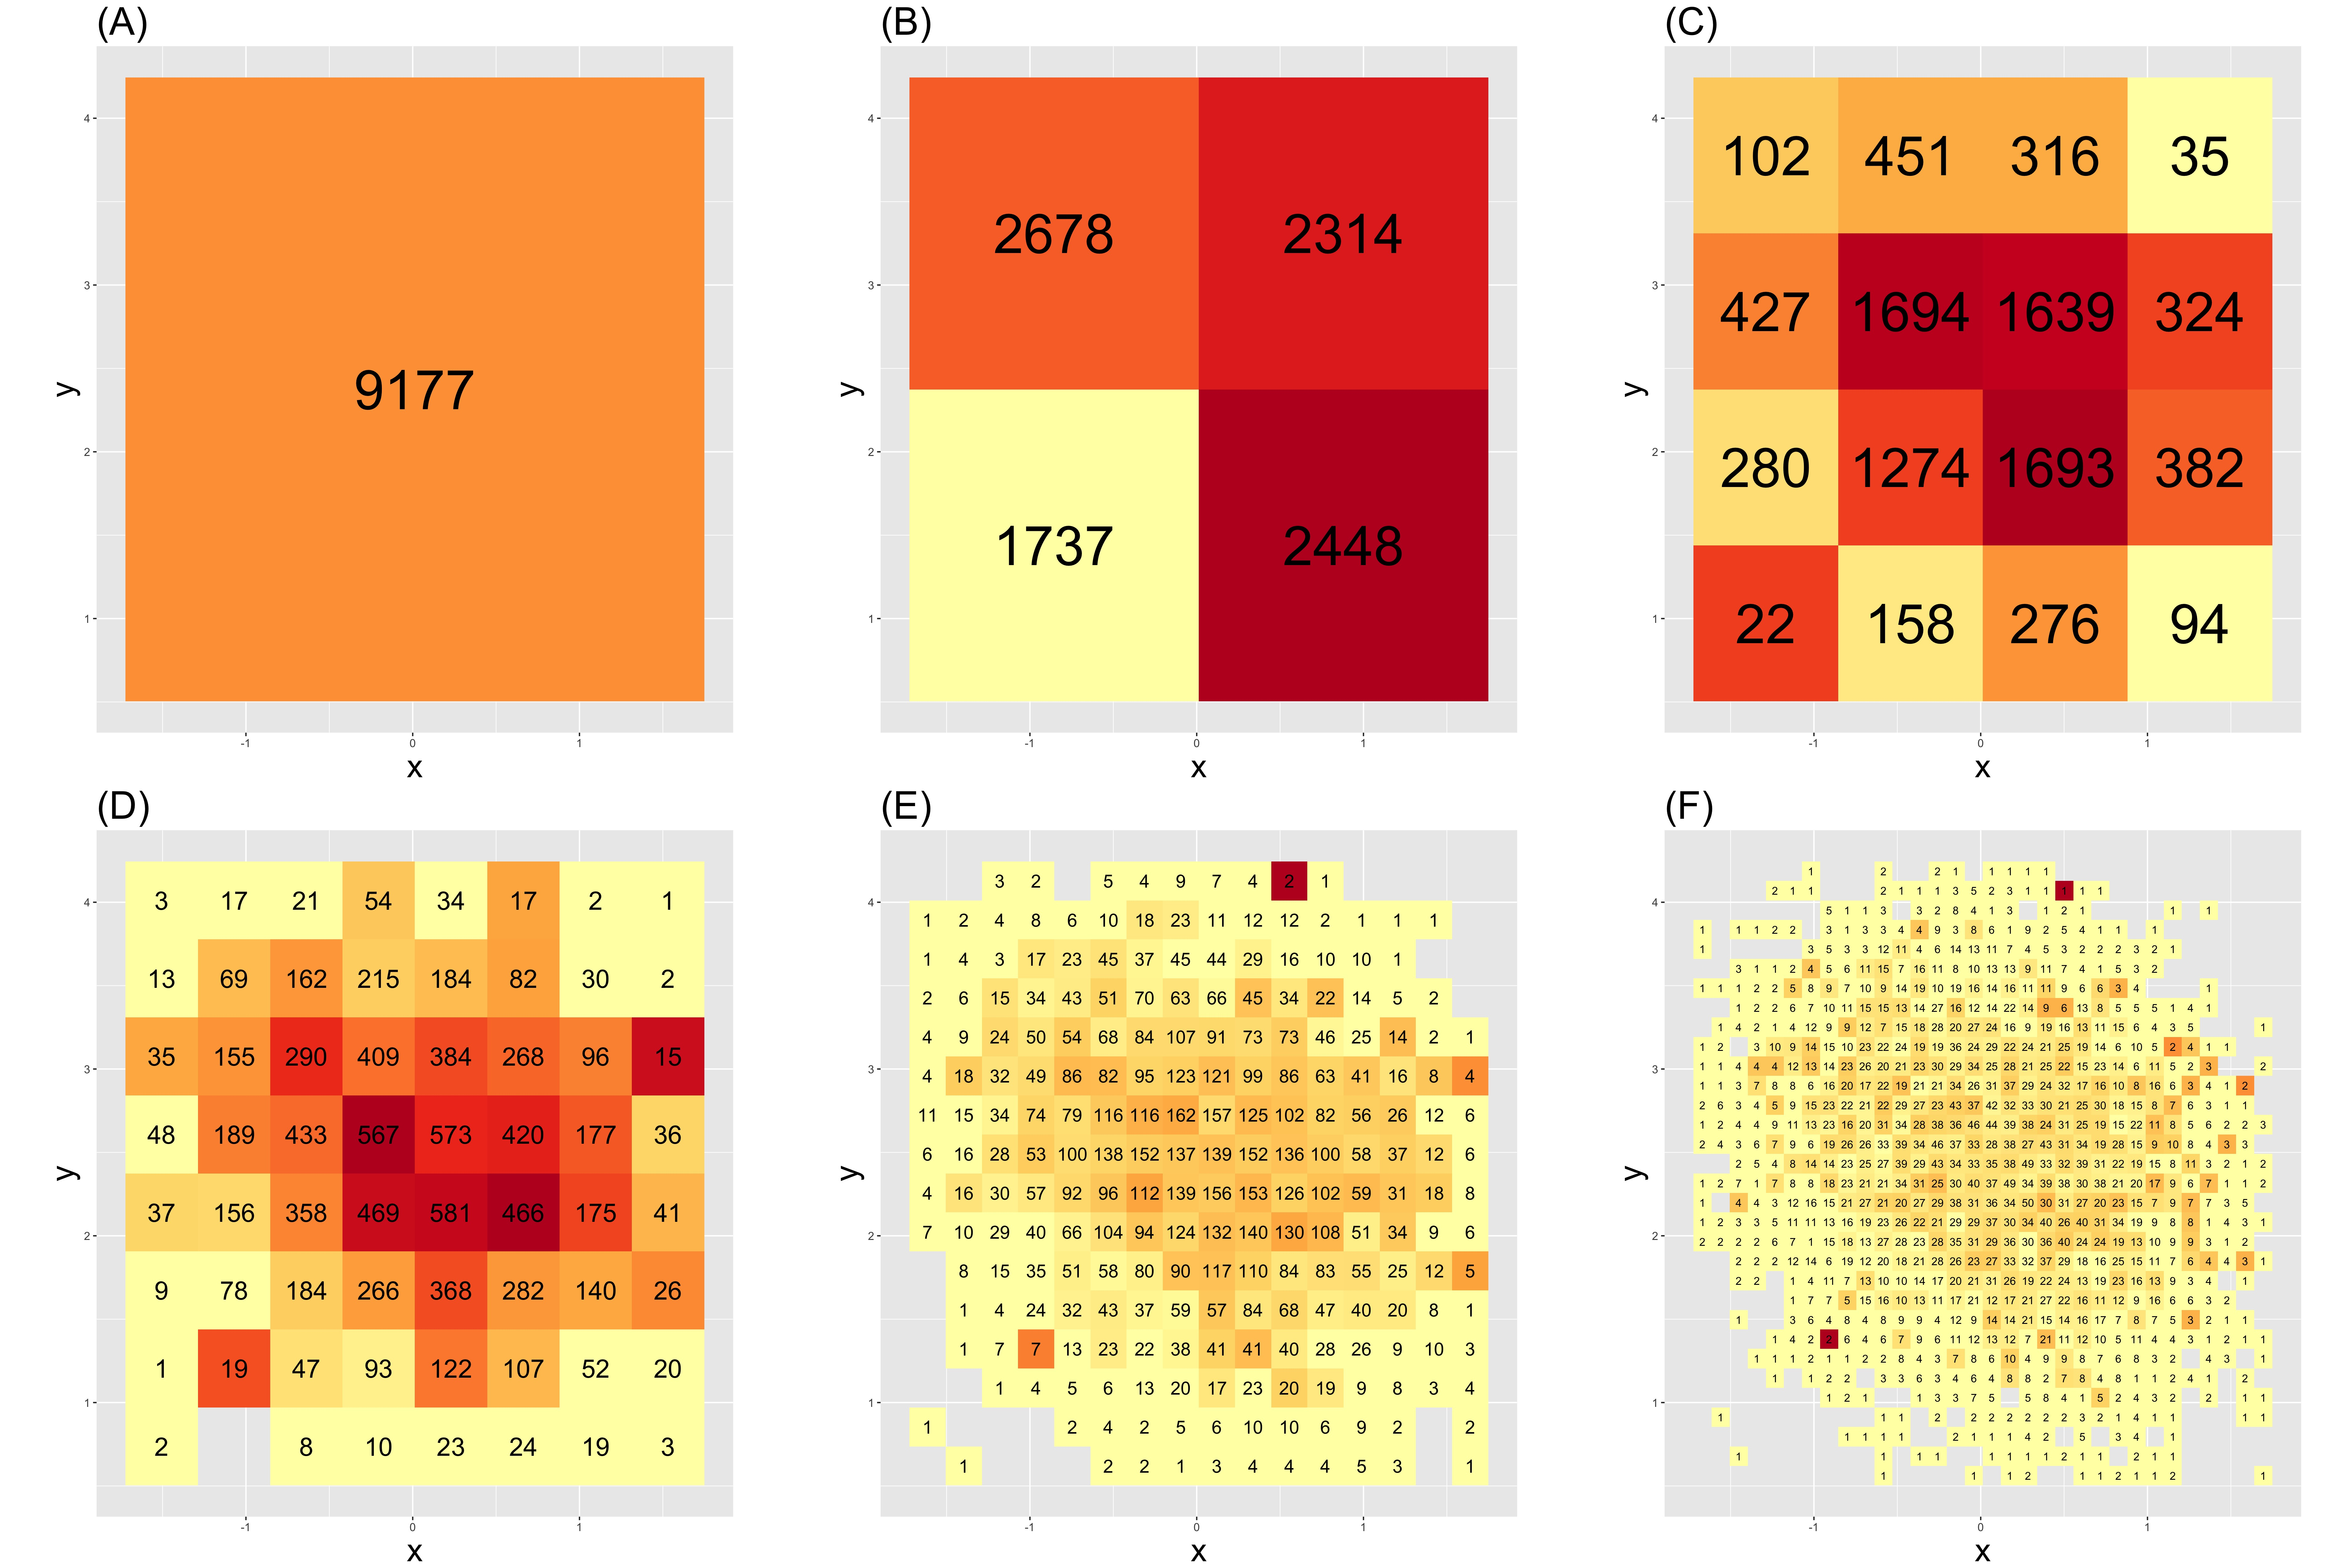
\includegraphics[scale=.4]{Images/Chapter_VarRes.png} 
      	\caption{These {\bf six (?)} heat maps show the same data, 9177 swings by batter 425509, Johnny Peralta, at increasing resolutions. Heat map one is unnecessarily coarse, while heat map six is excessively fine. Note how dramatically the visual imact and impression varies as the resolution increases. Which resolution best conveys the data?}
      	\end{figure} 

It is unclear which of these five resolutions best combines spatially precise estimates of $p$ where possible, and box sample sizes with $\text{Var}(\hat{p}_{b})$ in a desirable range. The viewer interested in the center of the strike zone should prefer the last ({\bf need labels} heat map, as the box sample sizes are sufficient to provide such spatially specific low variance estimates. The boxes closer to the edges of the strike zone contain higher variance, and thus less reliable estimates, due to prohibitively small sample sizes. We propose a new heat map approach that combines resolutions according to the data's varying spatial density.

\subsection{Empirical Heat Maps and Spatially Varying Resolution} % ==========

Consider again the heat map in Figure 2. Notice box (1,1) contains data on 22 swings, a sample size where subdividing would yield sample sizes uselessly small, and thus estimate variances prohibitively high. Box (2,3), in contrast, contains data on 1694 swings, which would support estimates that are more spatially accurate without $\text{Var}(\hat{p}_{b})$ increasing past acceptable levels. We propose defining a stopping rule and a subdividing method, and subdividing boxes further accordingly. For example, in Figure 4 we subdivide, into four equally sized boxes, all boxes where $n_{b} > 200$, . One iteration through all boxes at their current size, subdividing according to this rule, converts the heat map on the left to the heat map on the right.
        \begin{figure}[H]
      	\centering
      	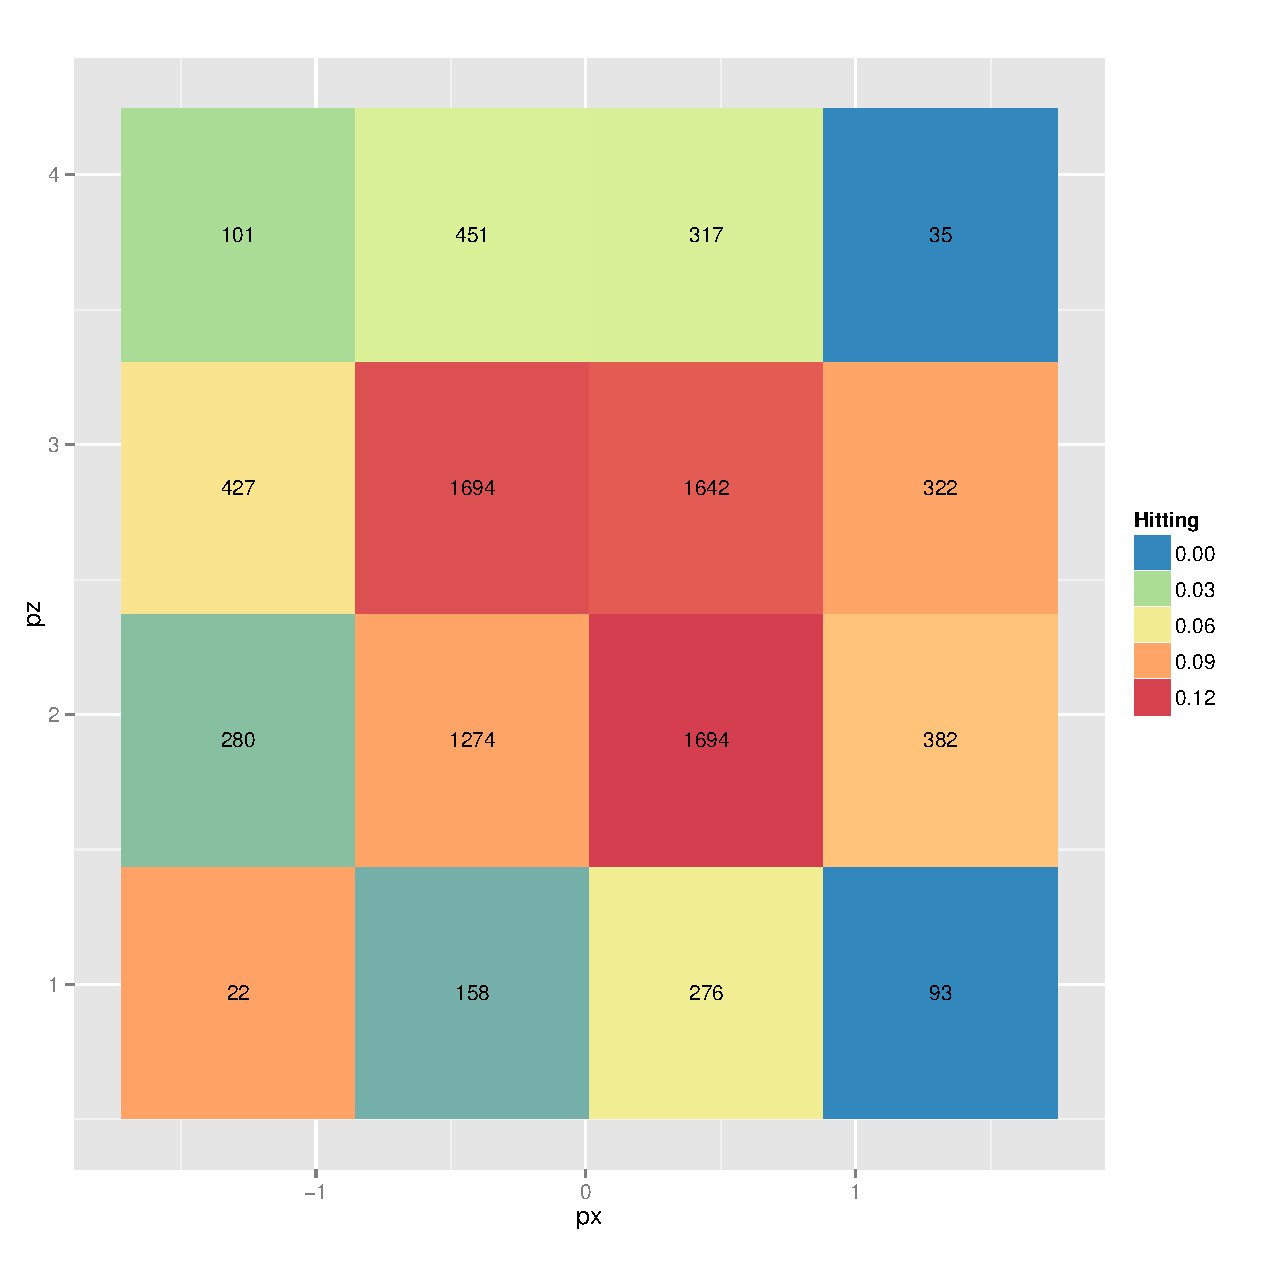
\includegraphics[scale=.3]{Images/Chapter4x4.pdf} 
      	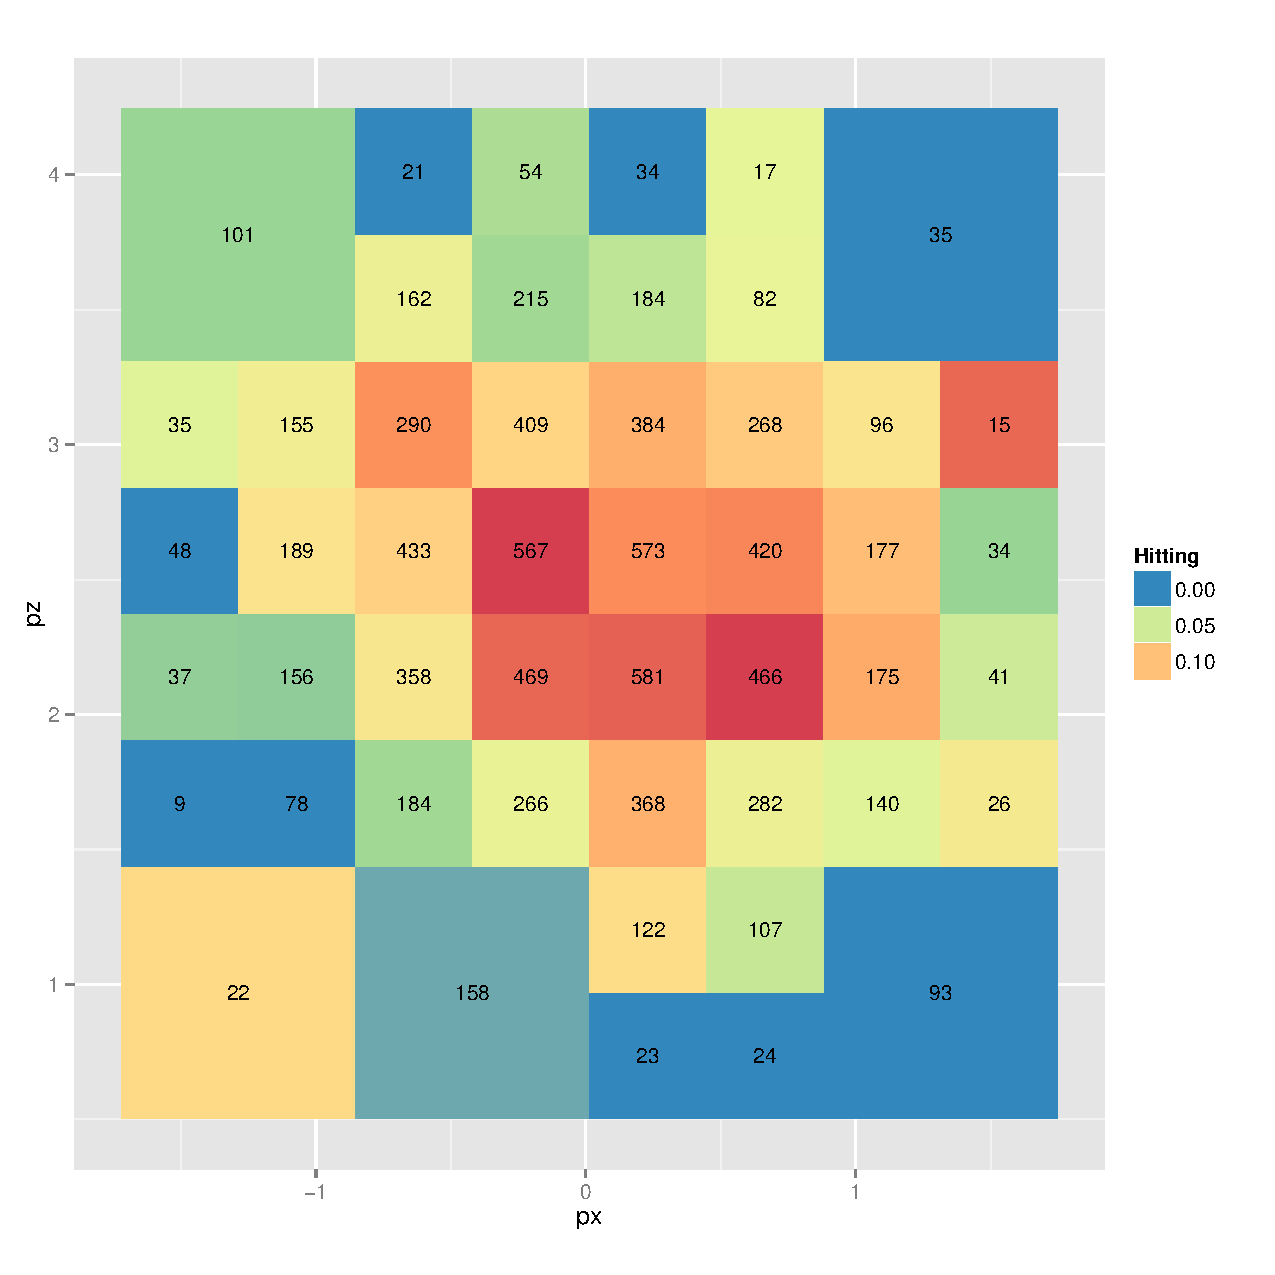
\includegraphics[scale=.3]{Images/Chapter8x8_200.pdf} 
      	\caption{These heat maps convey the empirical batting average of Johnny Peralta in each square region of the hitting zone. Each box maps $\hat{p}_{b}$ to a color. The number printed on each box represents the number of pitches Peralta swung at that passed through that box. Notice that all boxes with a sample size greater than 200 in the heat map on the left, have been subdivided in the heat map on the right.}
      	\end{figure} 
Notice all four corner boxes have not subdivided, indicating Peralta seldom sees and swings at pitches in these locations. The boxes toward the middle of the map tend to have larger sample sizes, and higher $\hat{p}_{b}$. Pitches pass through the middle of the hitting zone more frequently because many pitch target margin of error circles overlap there; and it is the region where pitch target margin of error circles are entirely inside the strike zone. Sixteen boxes still have a sample size greater than 200, and 11 still have a sample size greater than 300. We iterate again, and further subdivide 16 boxes where $n_{b} > 200$.
        \begin{figure}[H]
      	\centering
      	
      	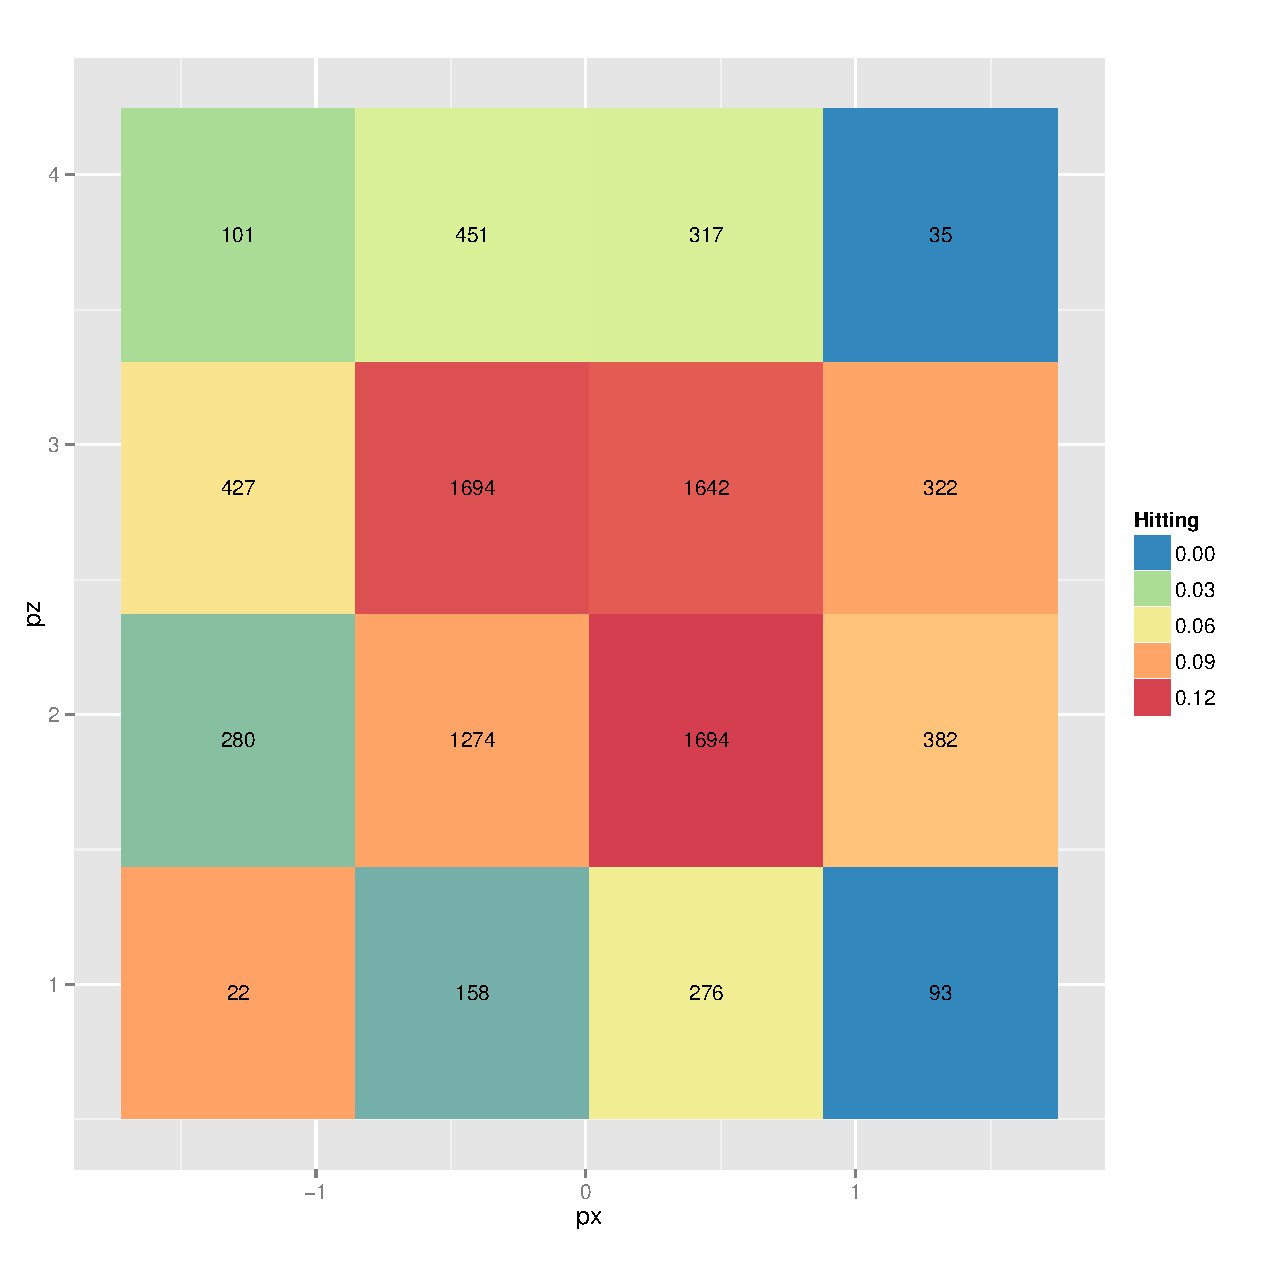
\includegraphics[scale=.25]{Images/Chapter4x4.pdf}
      	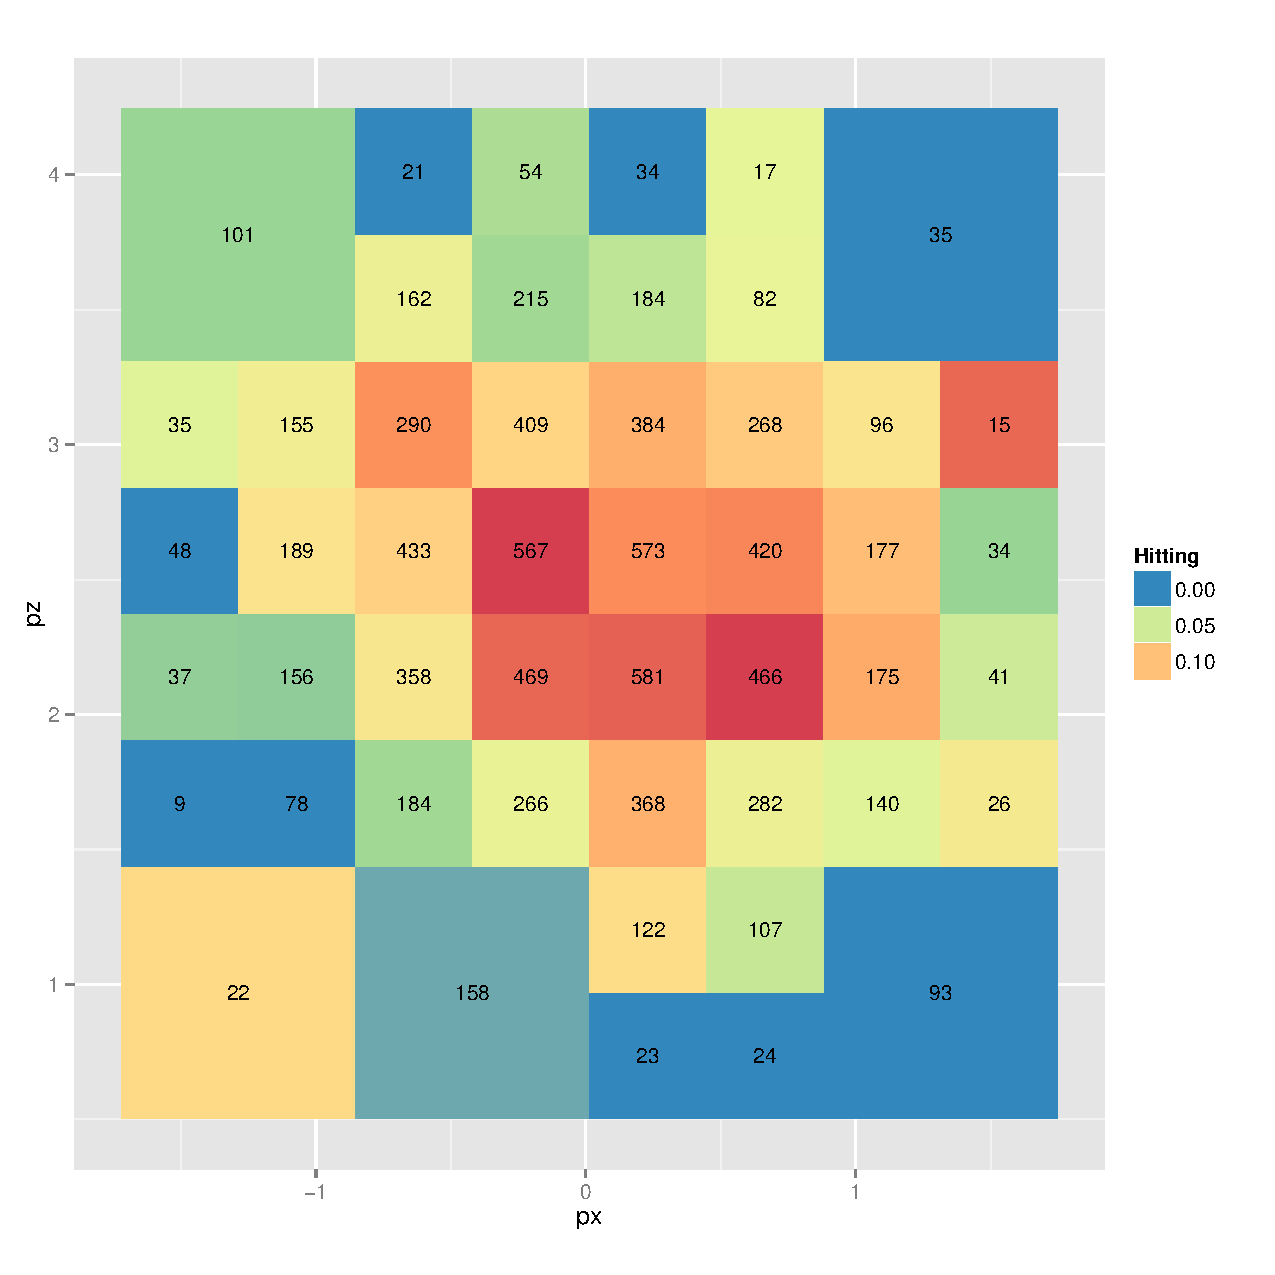
\includegraphics[scale=.25]{Images/Chapter8x8_200.pdf} 
      	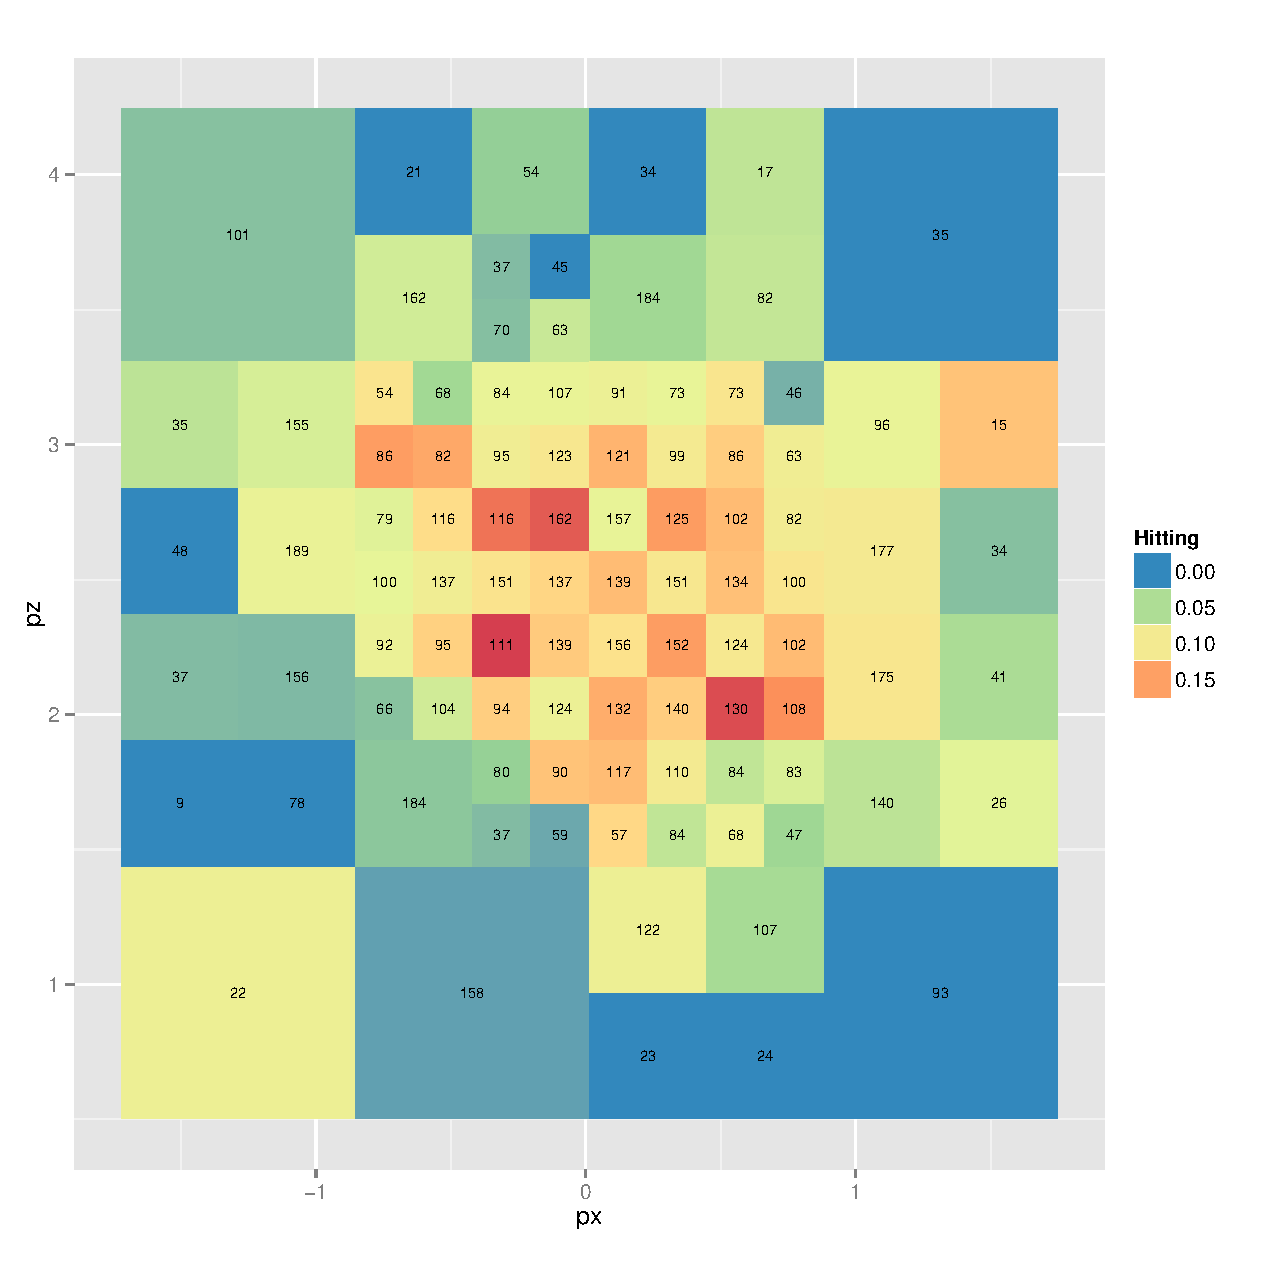
\includegraphics[scale=.25]{Images/Chapter16x16_200.pdf} 
      	\caption{These heat maps convey the empirical batting average of batter 425509, Johnny Peralta, in each boxed region of the hitting zone. Each box maps $\hat{p}_{b}$ to a color. The number printed on each box represents the number of pitches the hitter swung at that passed through that box. All boxes with a sample size greater than 200 in the heat map on the left, have been subdivided in the heat map in the middle. All boxes with a sample size greater than 200 in the heat map in the middle, have been subdivided in the heat map on the right.}
      	\end{figure}
In Figure 6, the middle heat map has 16 boxes with $n_{b} > 200$. In the heat map on the right these 16 boxes have been subdivided into four boxes each. After this iteration, the heat map on the far right consists of 97 boxes, with a mean box sample size of 94.57, and median of 94. The minimum box sample size is 9, and the maximum is 189. The first quartile box sample size is 63, and the third quartile is 125. Regions with a higher density of pitch-swings necessarily have smaller boxes, which acts to convey additional information to the reader, compared to a heat map on a uniform grid. Note that the stopping rule and subdivision algorithm can be defined by the map's creator, offering flexibility to create the heat map structure that suits the data. 

Figure 8 gives the full sequence of heat maps that result from applying the stopping rule $n_{b} < 100$, starting with a single box.
        \begin{figure}[H]
      	\centering
      	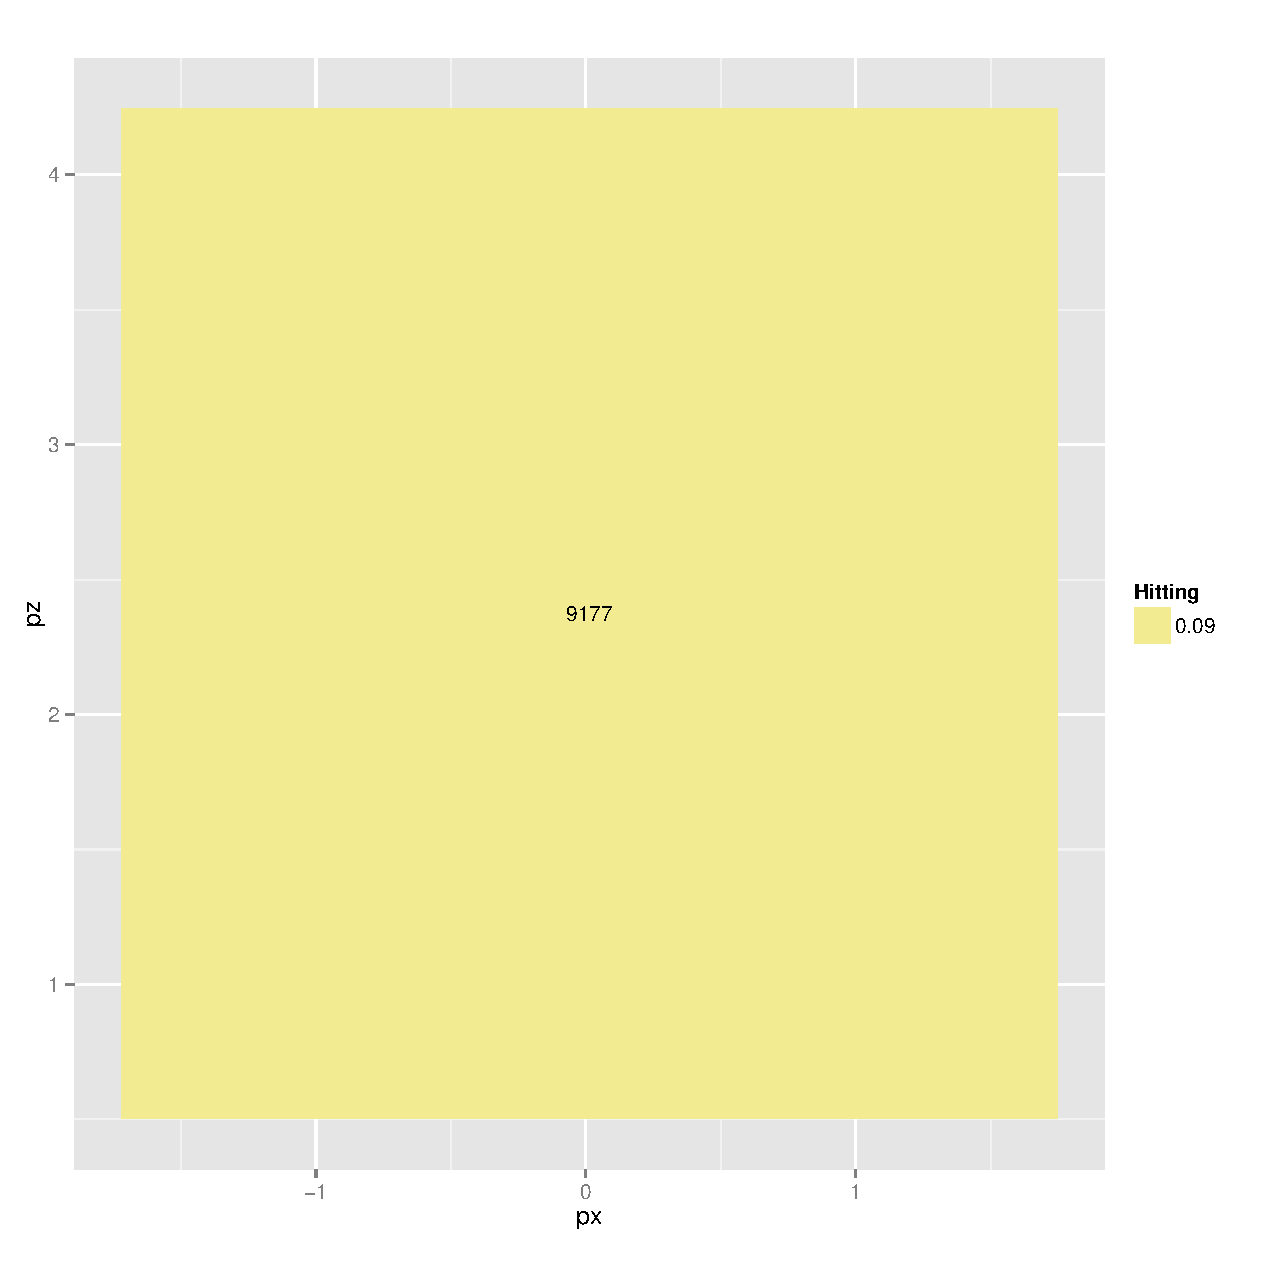
\includegraphics[scale=.2]{Images/Chapter1x1.pdf}
      	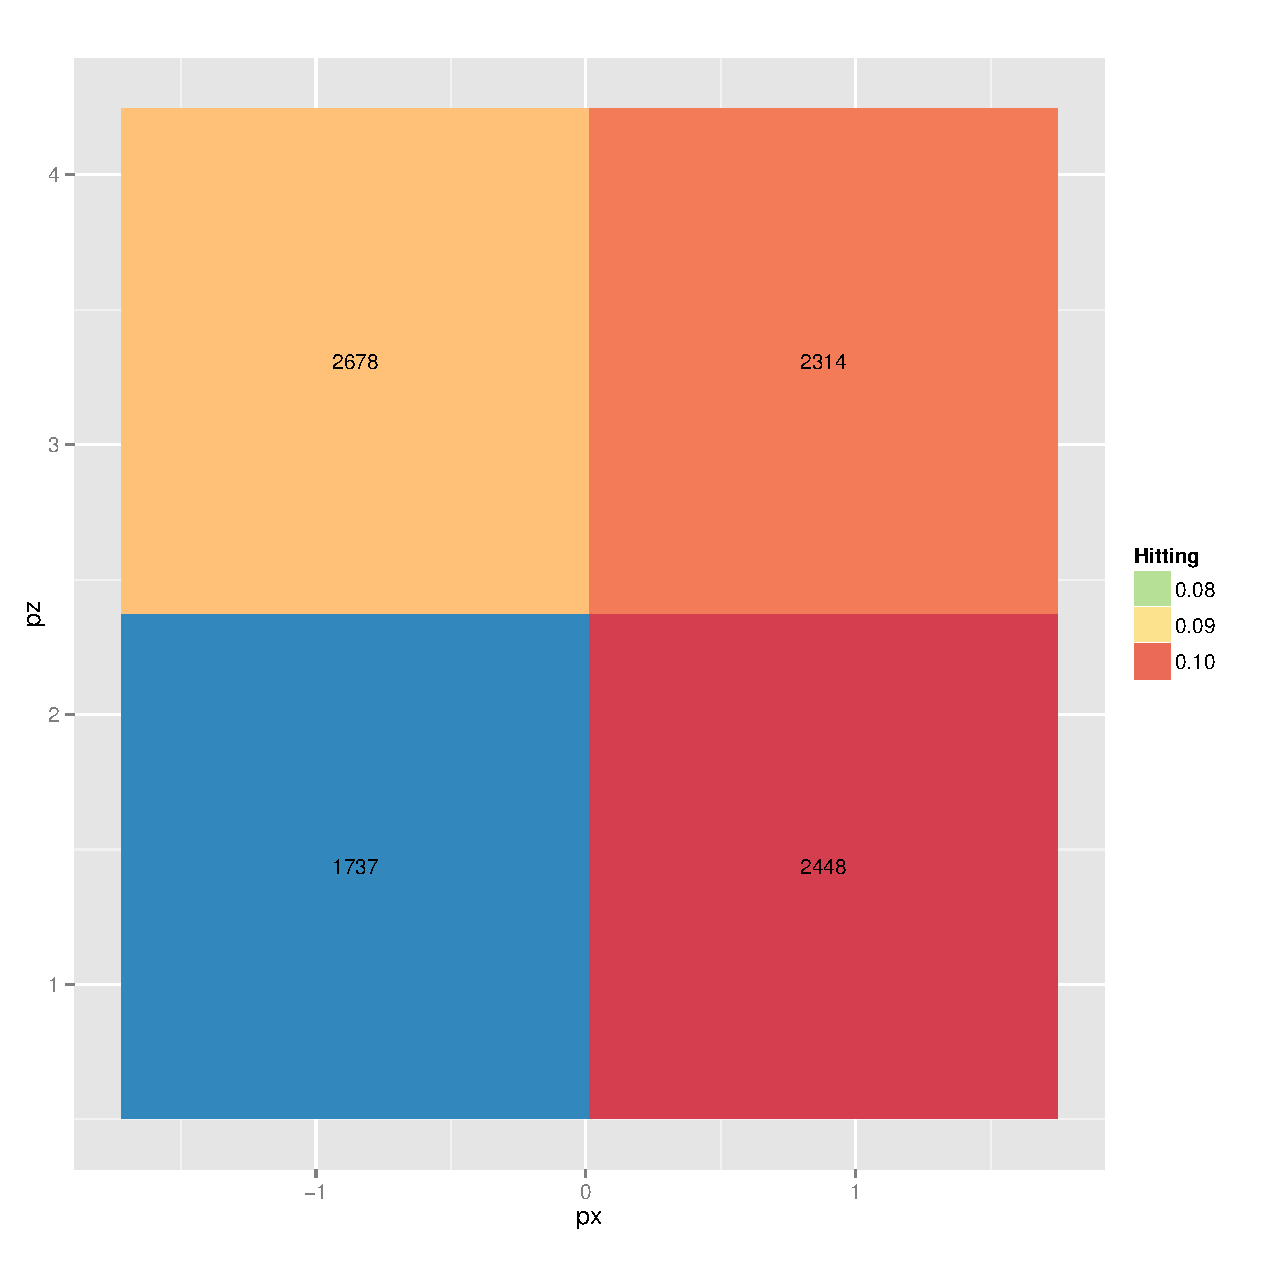
\includegraphics[scale=.2]{Images/Chapter2x2.pdf}
      	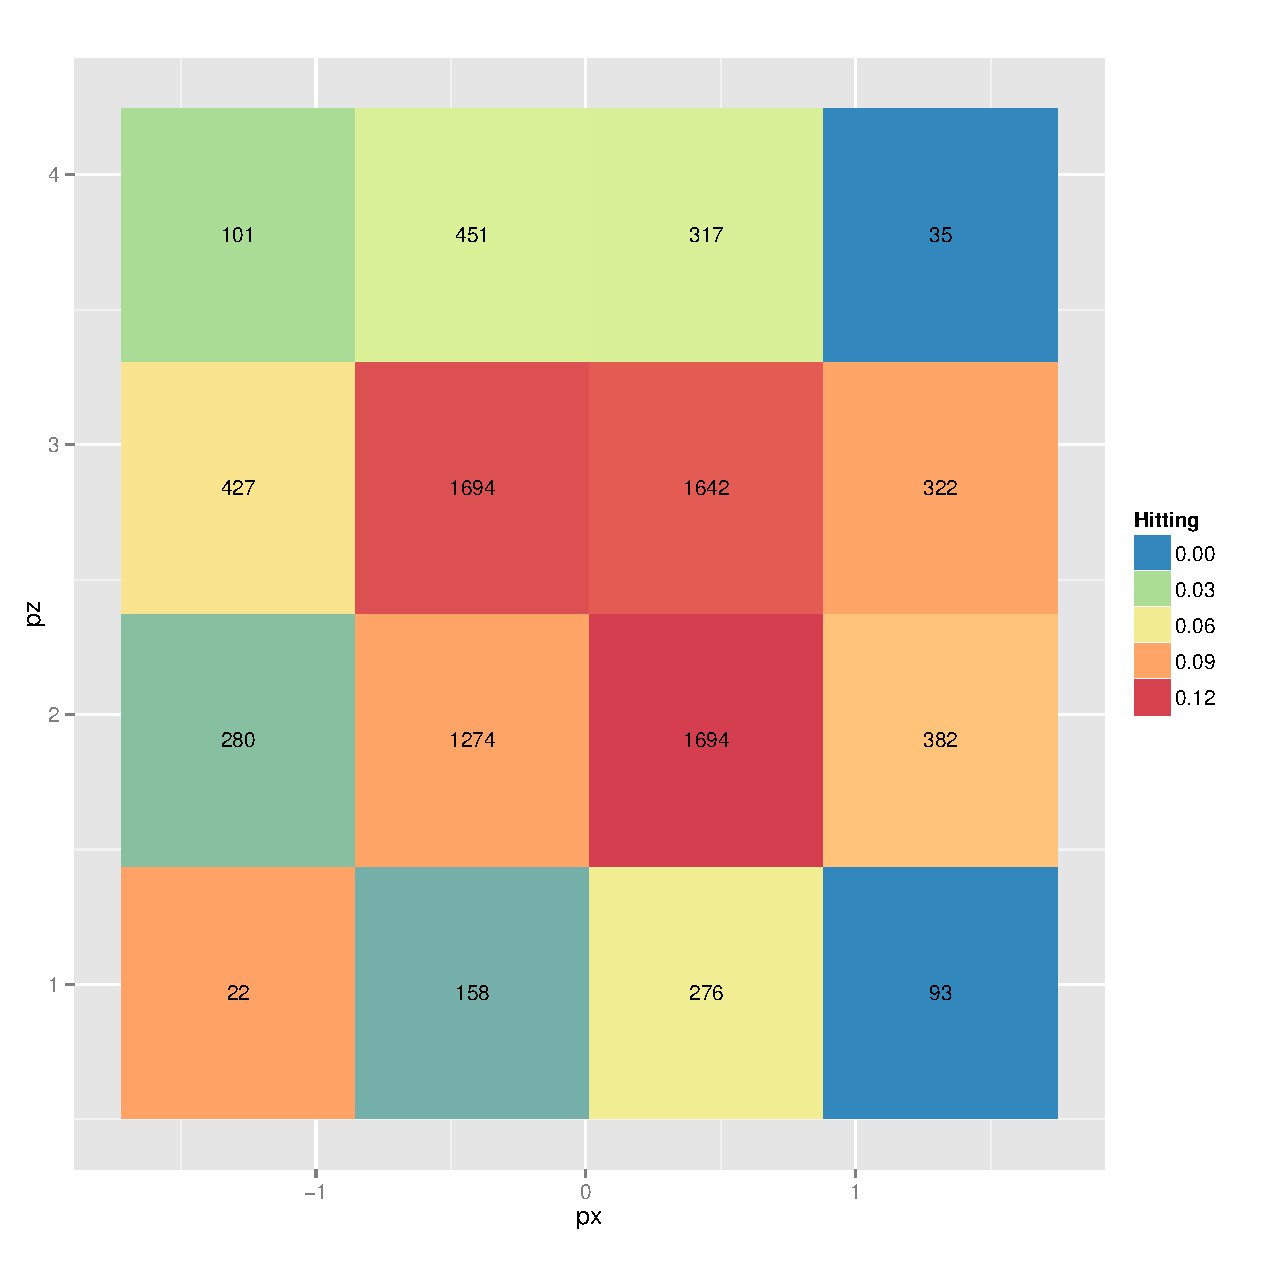
\includegraphics[scale=.2]{Images/Chapter4x4.pdf}
      	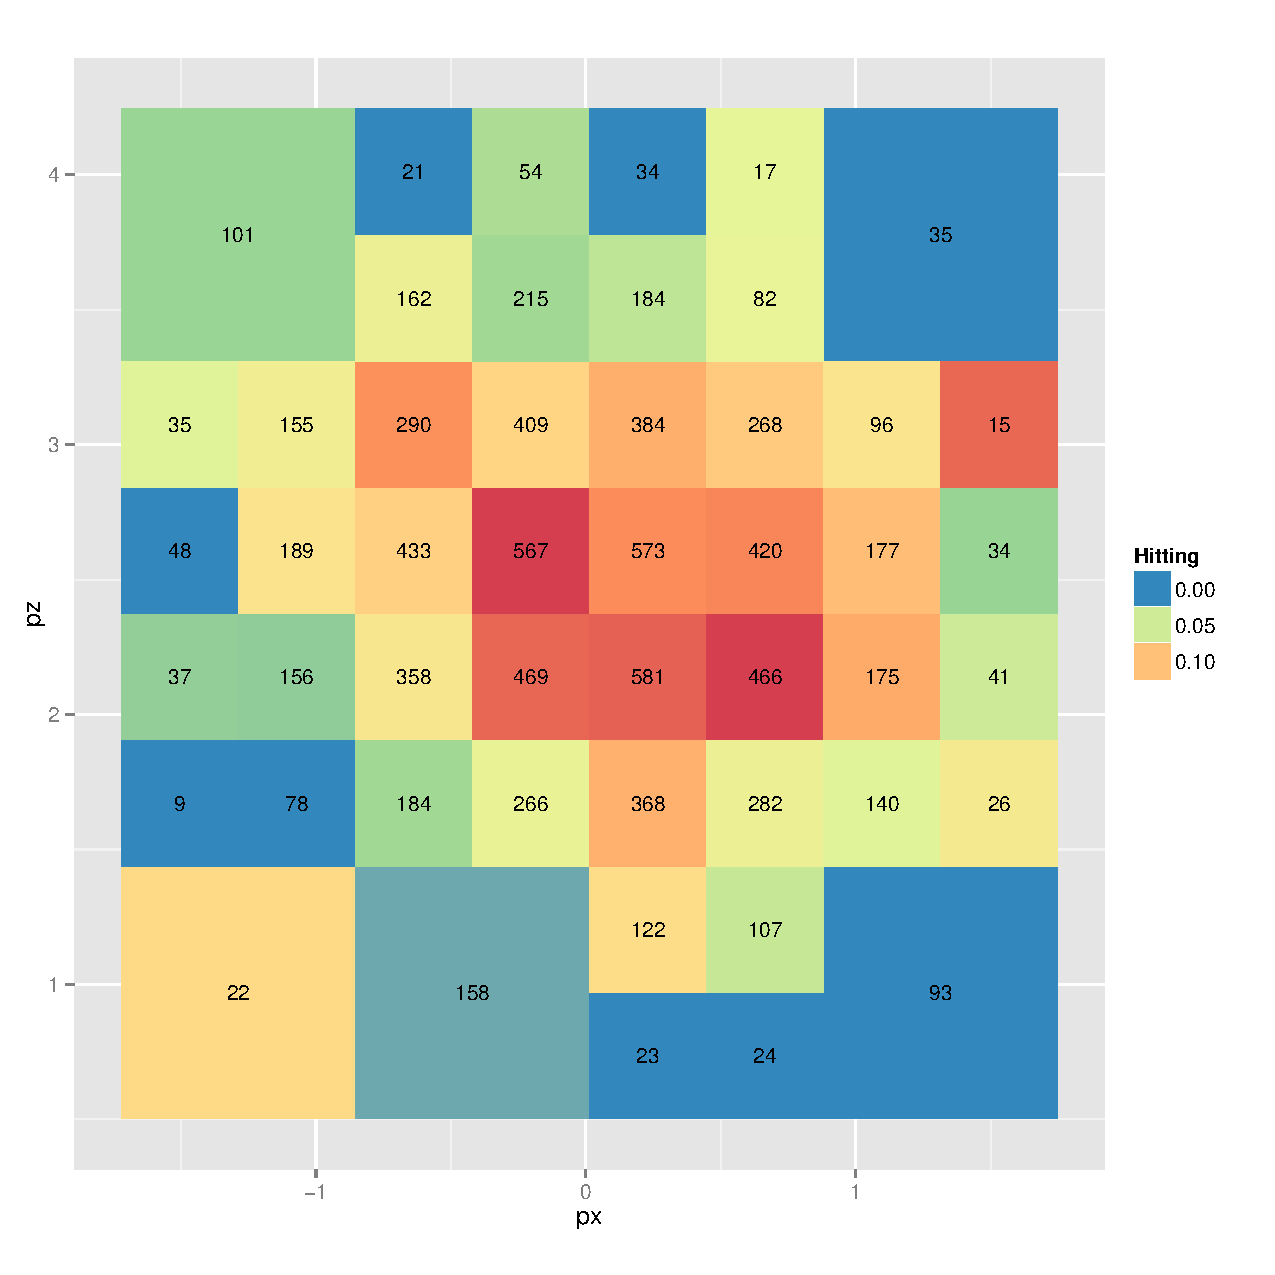
\includegraphics[scale=.2]{Images/Chapter8x8_200.pdf} 
      	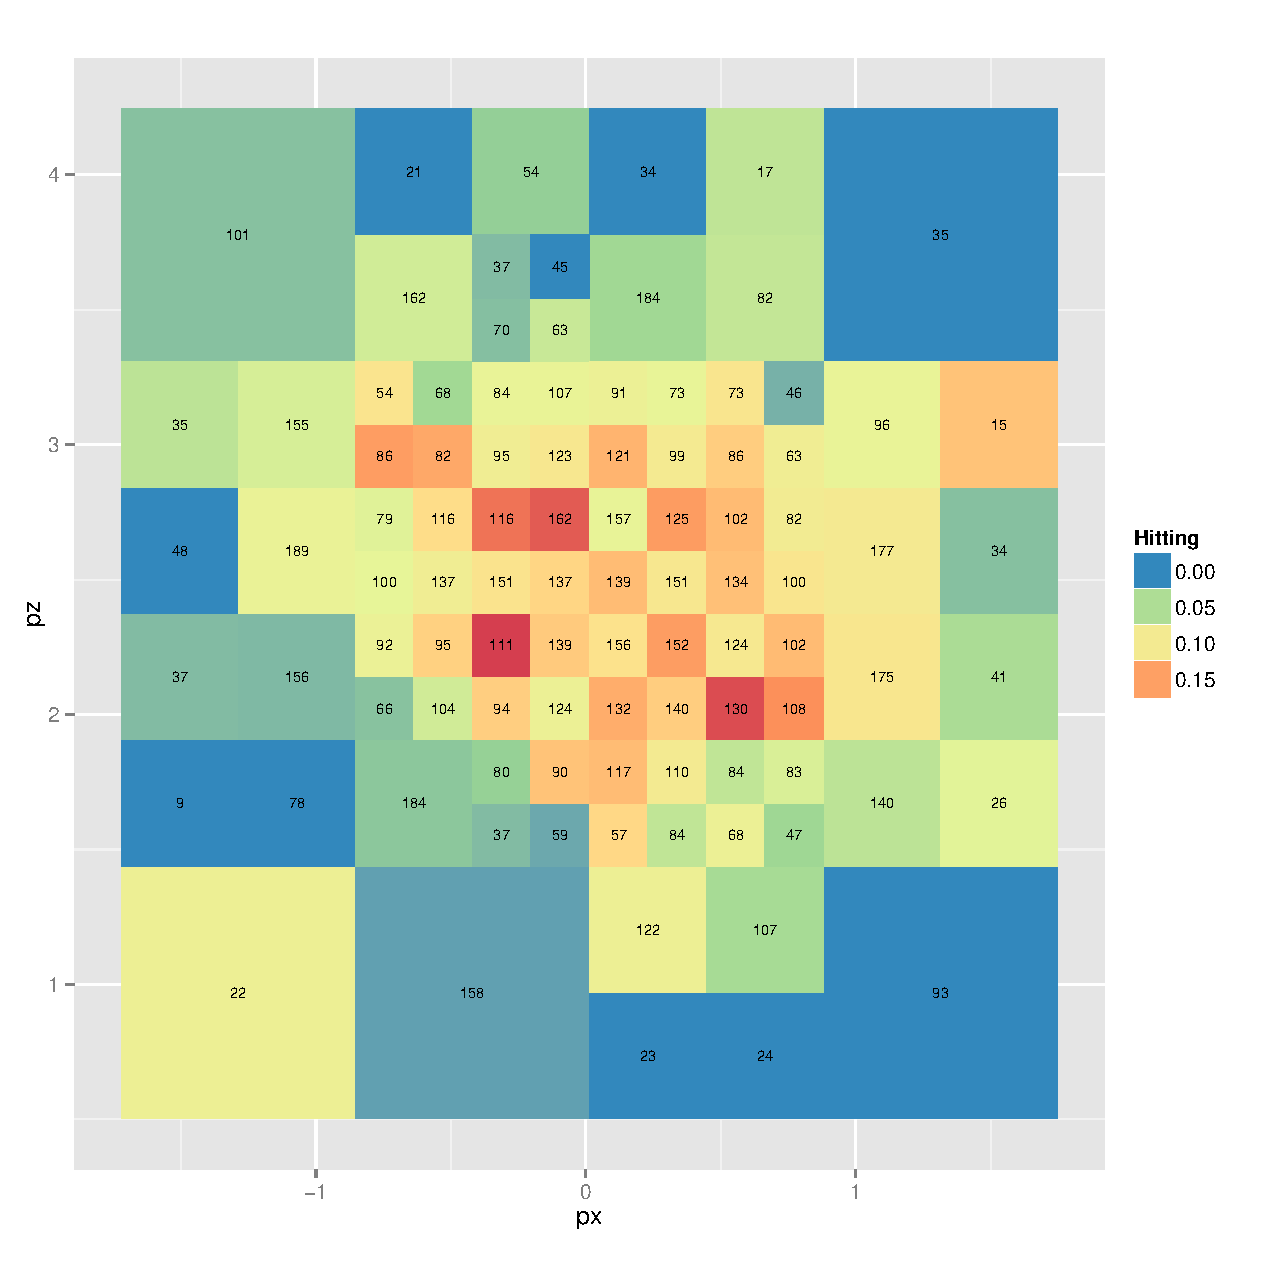
\includegraphics[scale=.2]{Images/Chapter16x16_200.pdf} 
      	\caption{These heat maps convey the empirical batting average of batter 425509, Johnny Peralta, in each boxed region of the hitting zone. Each box maps $\hat{p}_{b}$ to a color. The number printed on each box represents the number of pitches the hitter swung at that passed through that box. All boxes with a sample size greater than 200 in each heat map have been subdivided in the subsequent heat map.}
      	\end{figure}

To demonstrate the flexibility, consider a different stopping rule, $n_{b} < 100$. Figure 8 gives the sequence of heat maps that result from applying this stopping rule, with the same subdividing algorithm (***need to delineate what this algorithm is). 
        \begin{figure}[H]
      	\centering
      	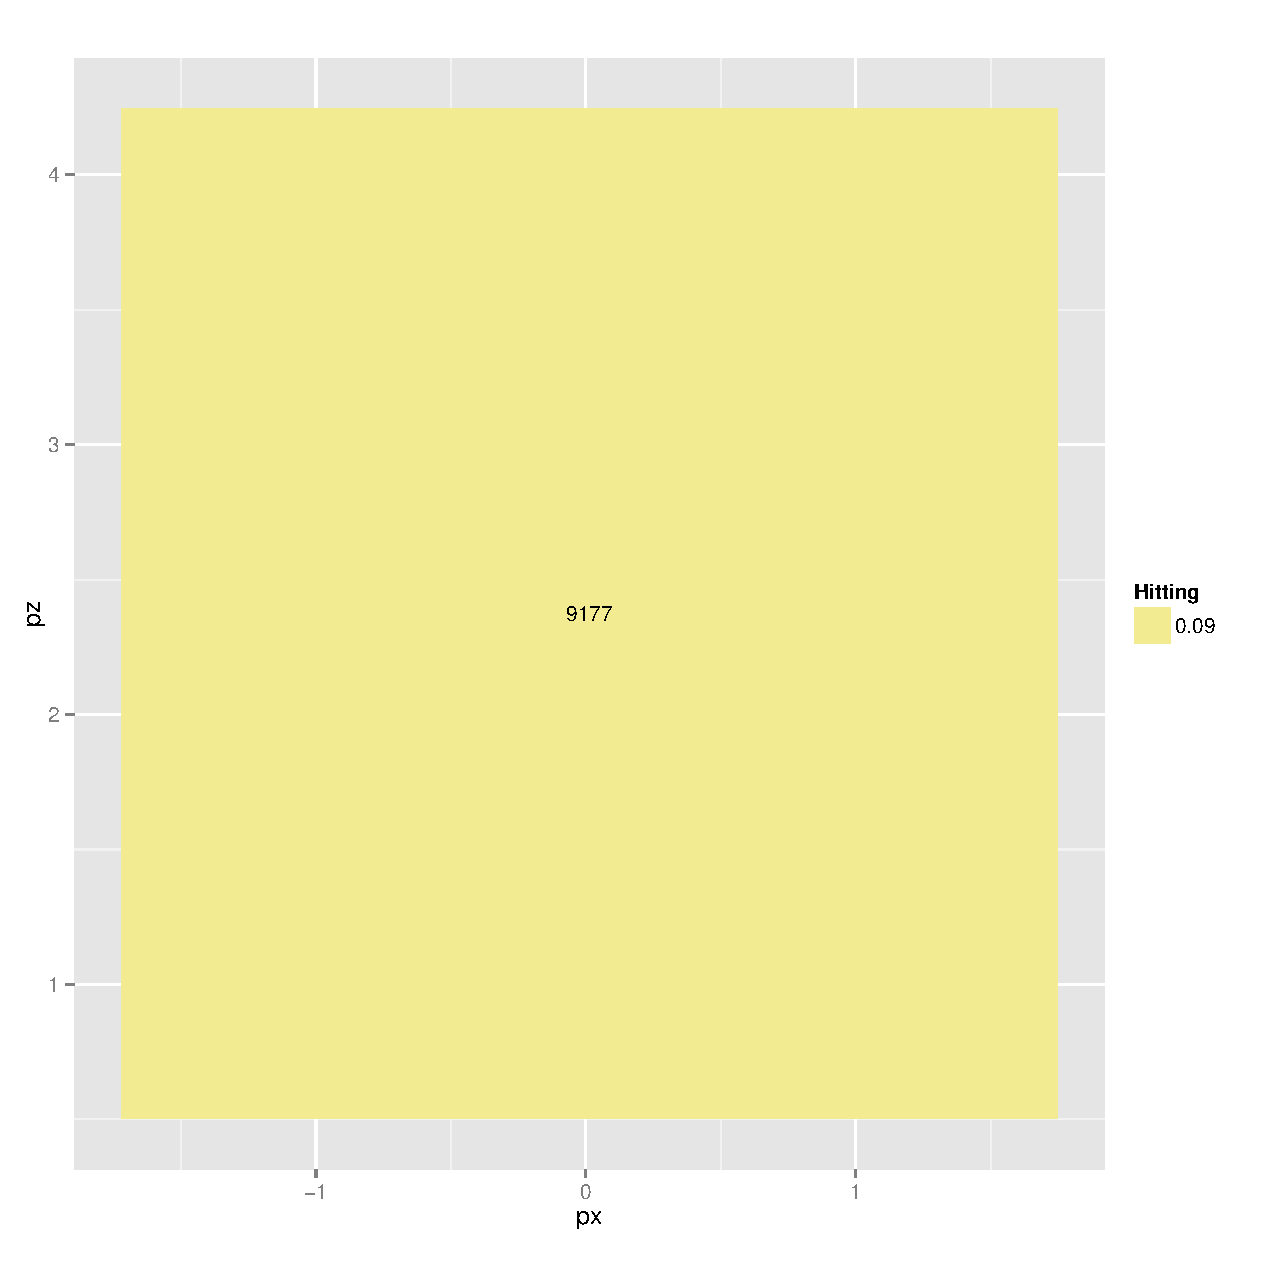
\includegraphics[scale=.2]{Images/Chapter1x1.pdf}
      	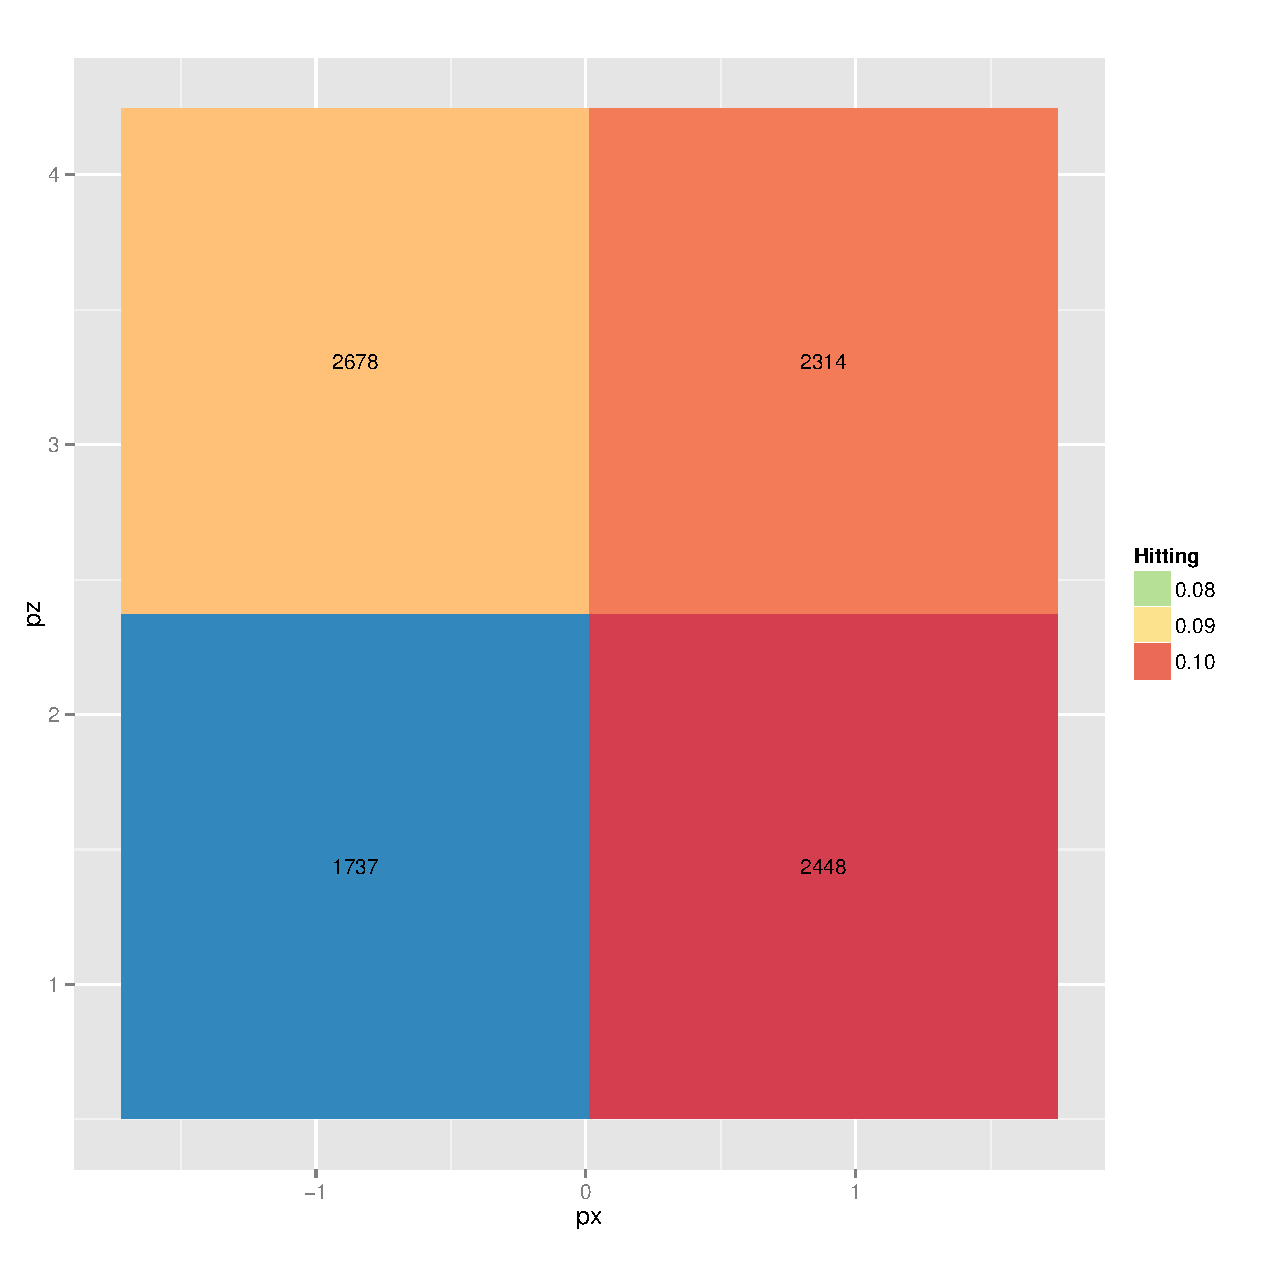
\includegraphics[scale=.2]{Images/Chapter2x2.pdf}
      	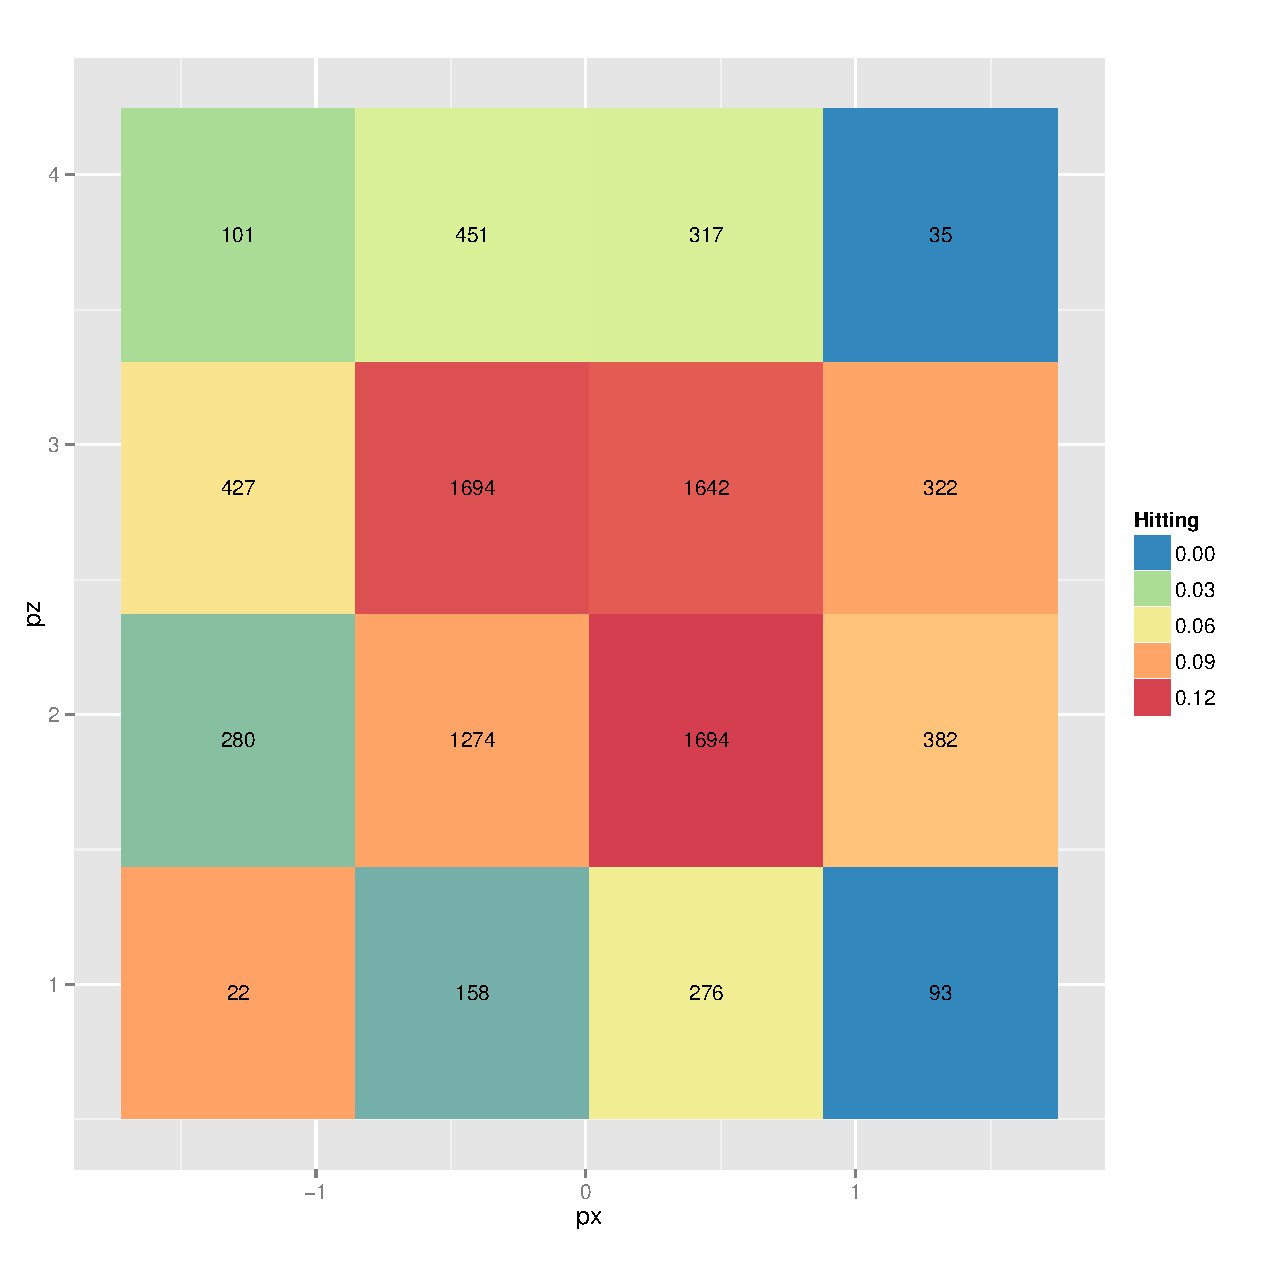
\includegraphics[scale=.2]{Images/Chapter4x4.pdf}
      	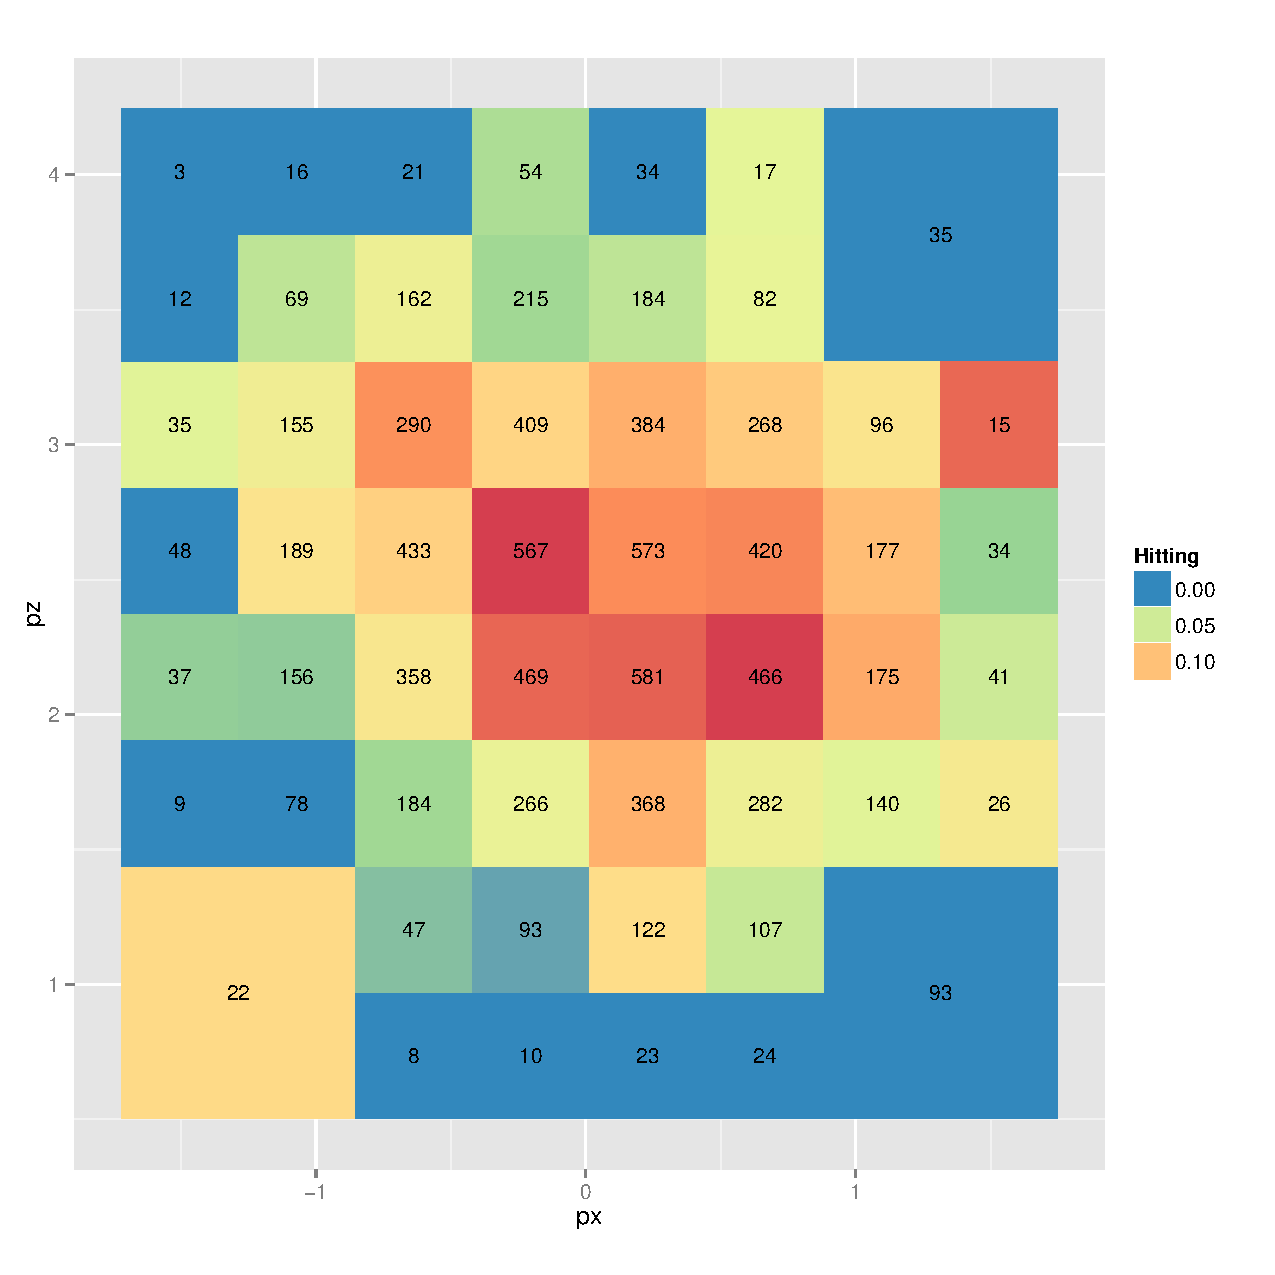
\includegraphics[scale=.2]{Images/Chapter8x8_100.pdf}
      	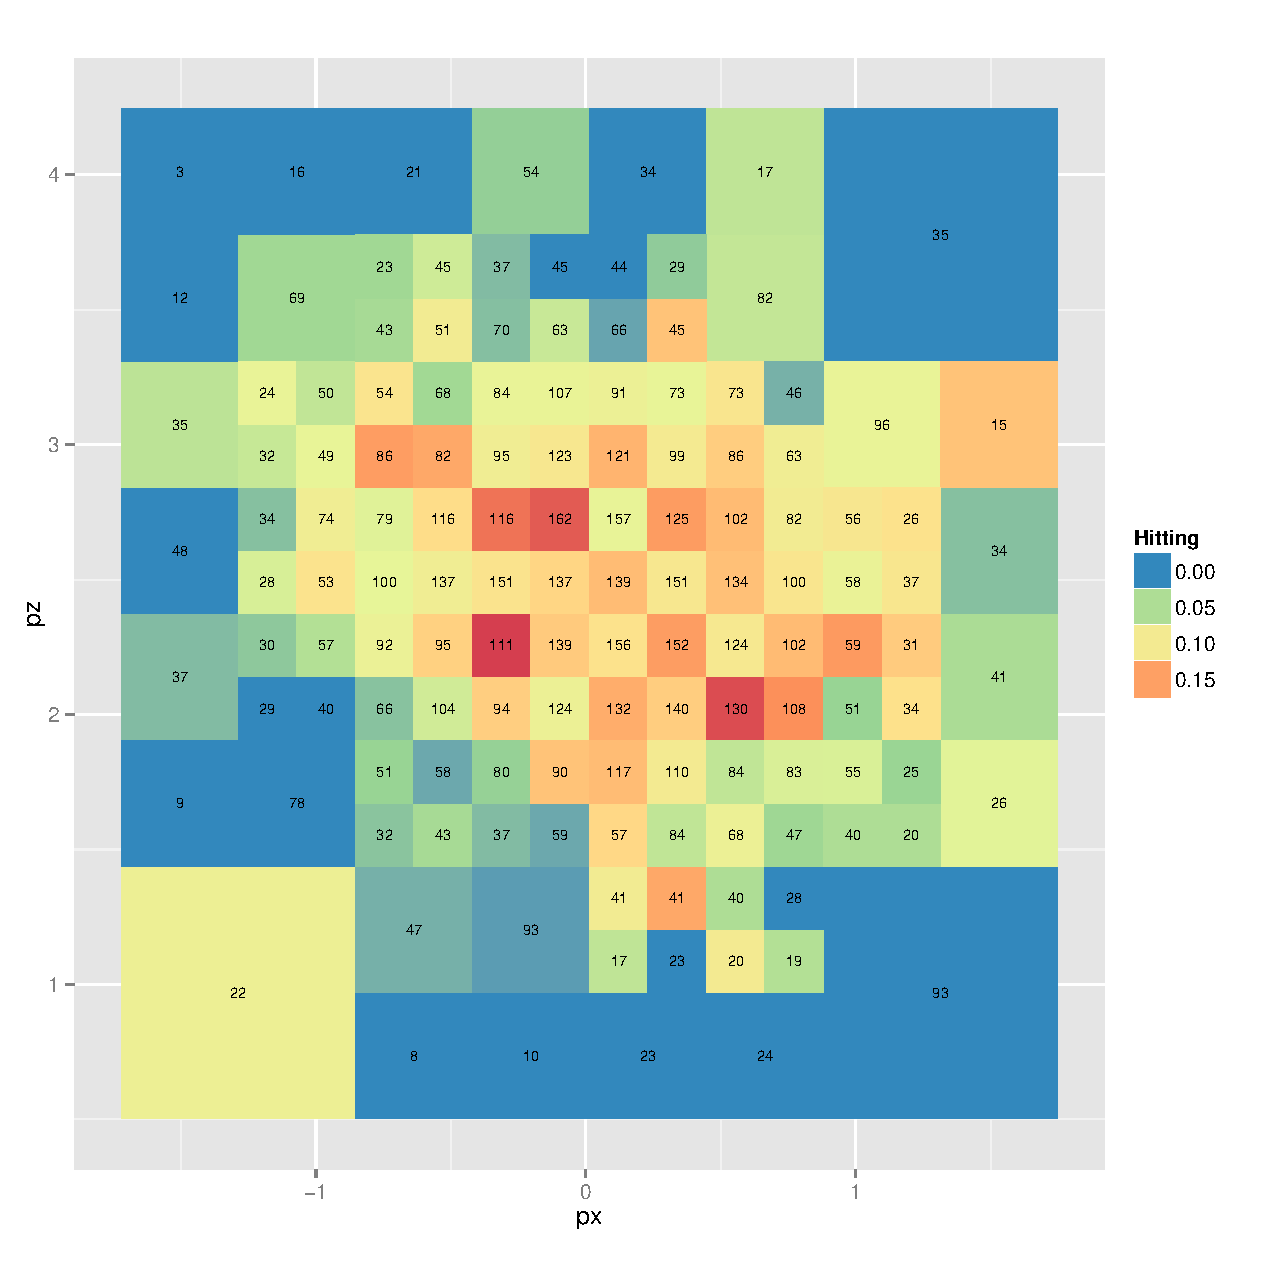
\includegraphics[scale=.2]{Images/Chapter16x16_100.pdf}
      	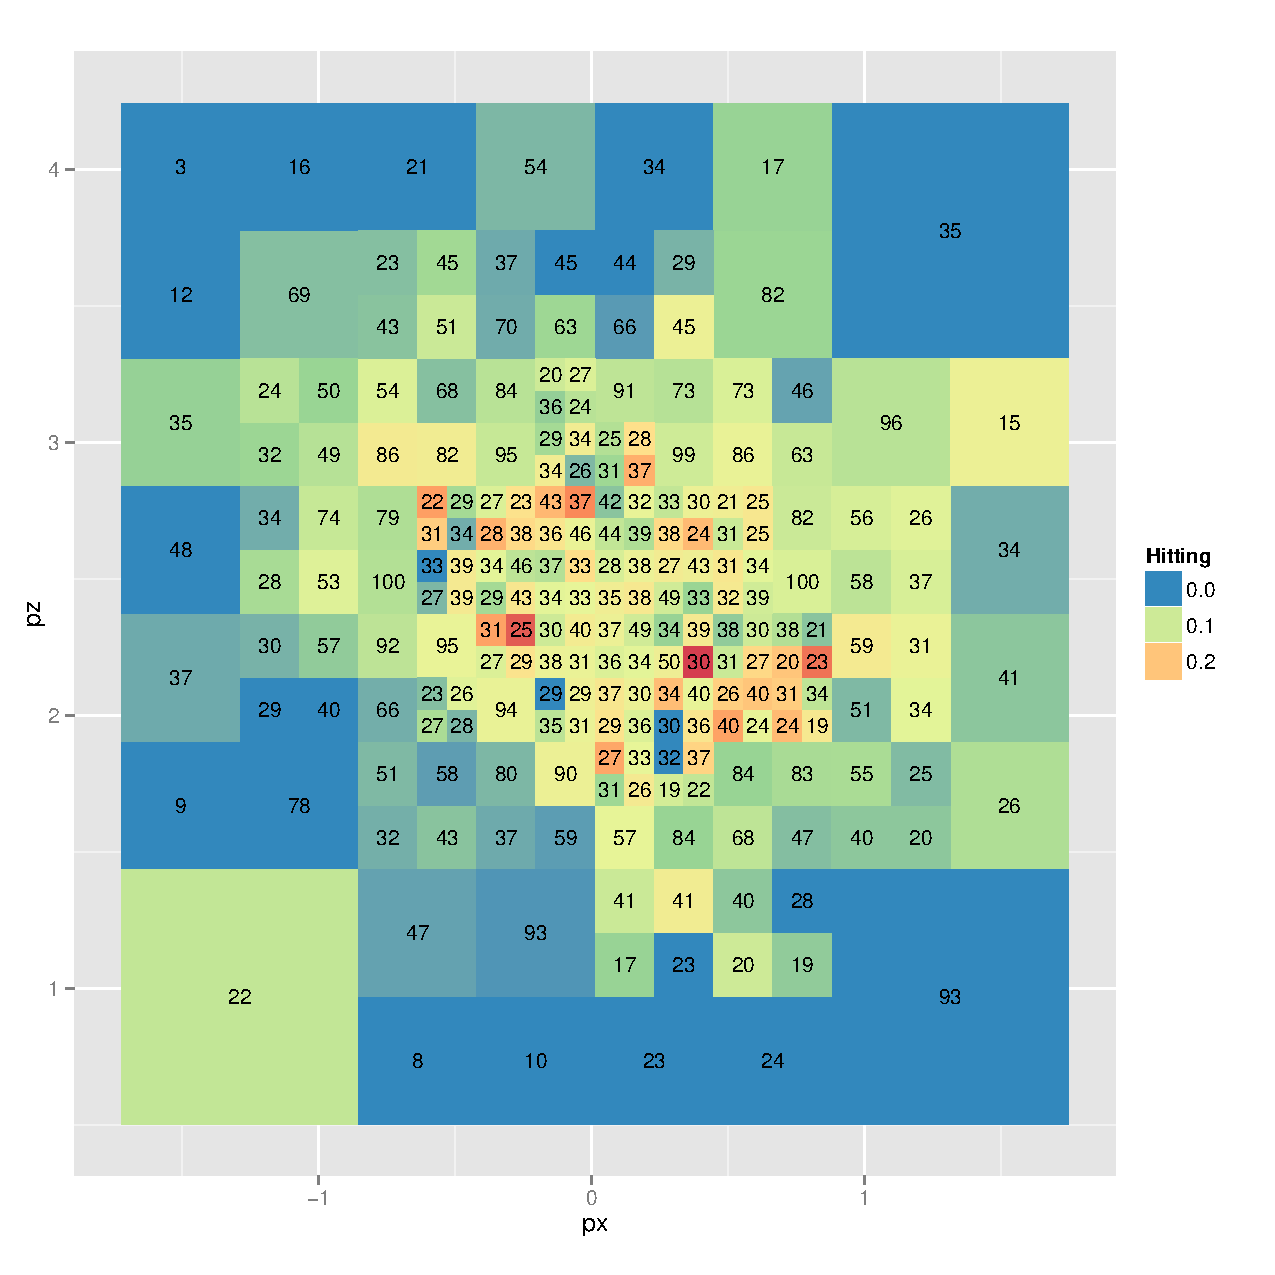
\includegraphics[scale=.2]{Images/Chapter32x32_100.pdf}
      	\caption{These heat maps convey the empirical batting average of batter 425509, Johnny Peralta, in each boxed region of the hitting zone. Each box maps $\hat{p}_{b}$ to a color. The number printed on each box represents the number of pitches the hitter swung at that passed through that box. All boxes with a sample size greater than 100 in each heat map have been subdivided in the subsequent heat map.}
\end{figure} 	
Compare this sequence to Figure 7, where the stopping rule was $n_{b} < 100$. The top row of heat maps in Figure 7 and Figure 8 are identical, but notice in the four by four heat map that $100 < n_{(2,1)} < 200, \text{ and } 100 < n_{(1,4)} < 200$. This implies one stopping rule applies, but the other does not.
        \begin{figure}[H]
      	\centering      
      	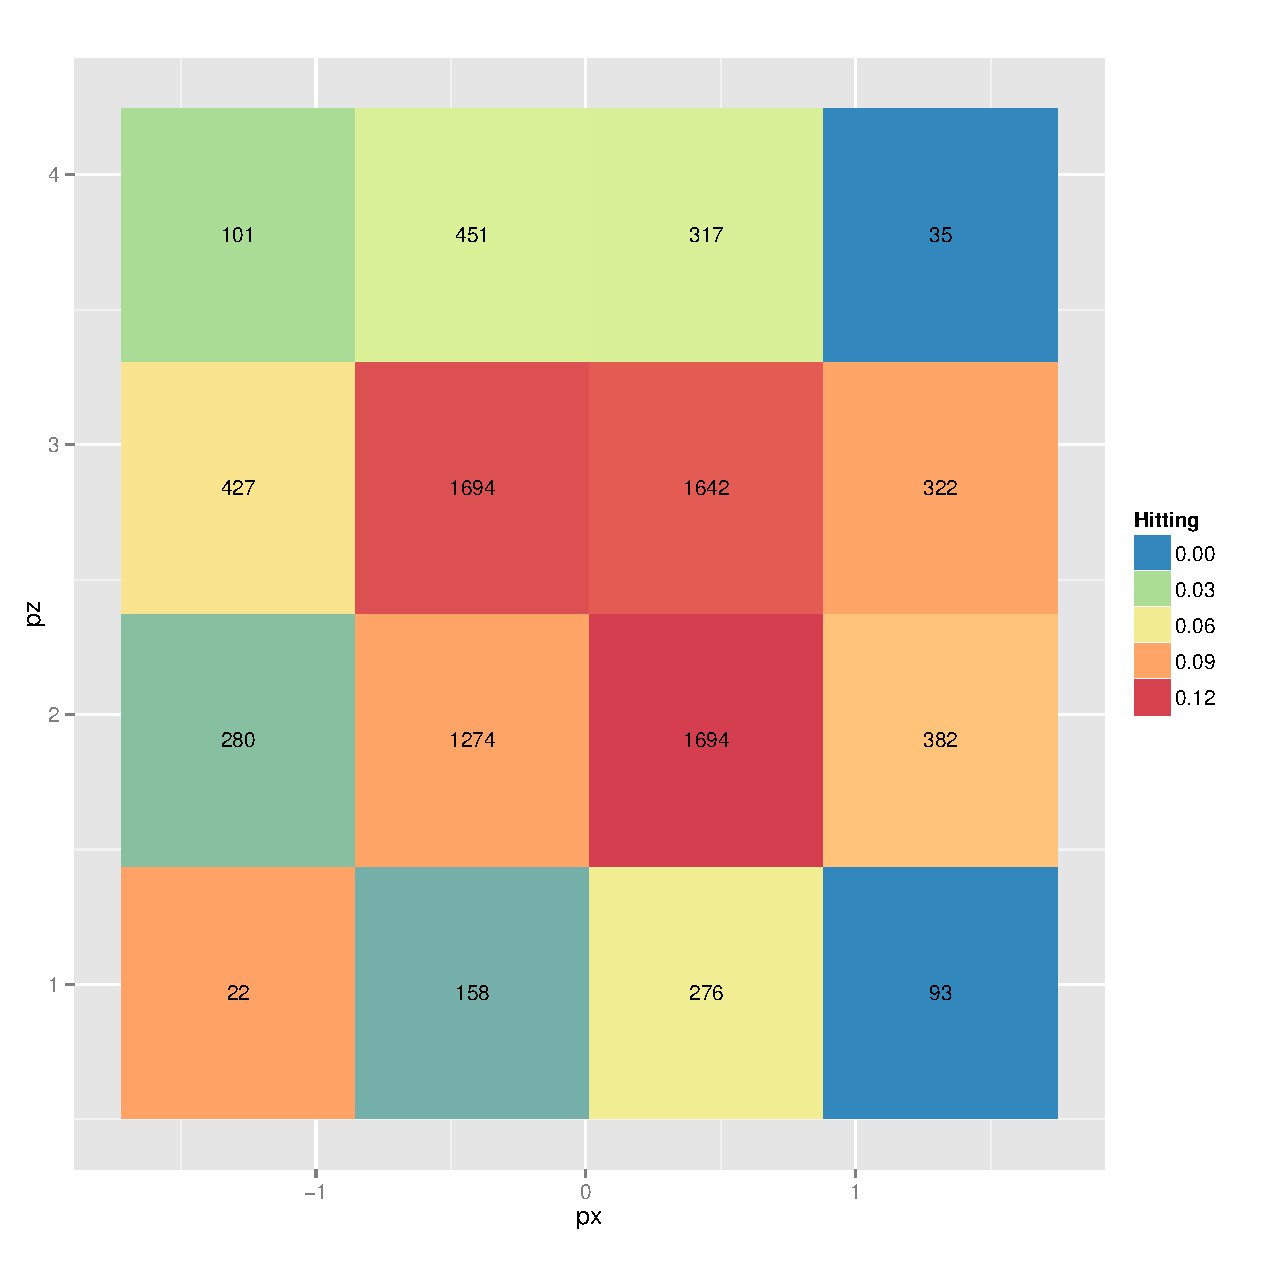
\includegraphics[scale=.2]{Images/Chapter4x4.pdf}
      	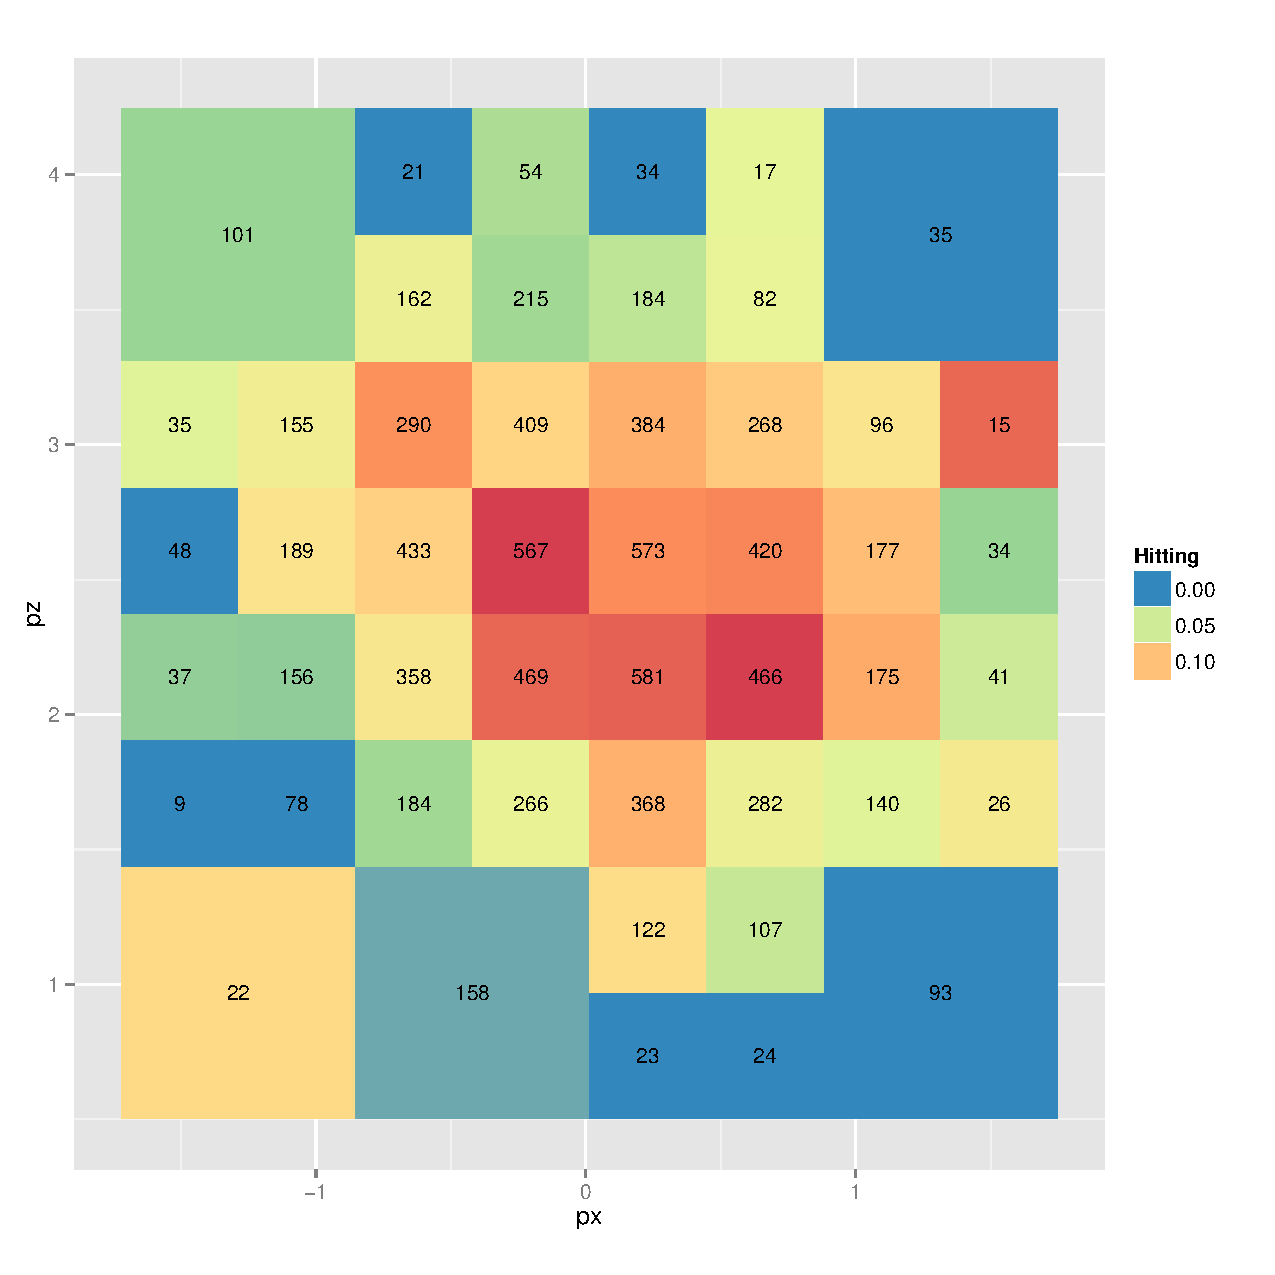
\includegraphics[scale=.2]{Images/Chapter8x8_200.pdf}
      	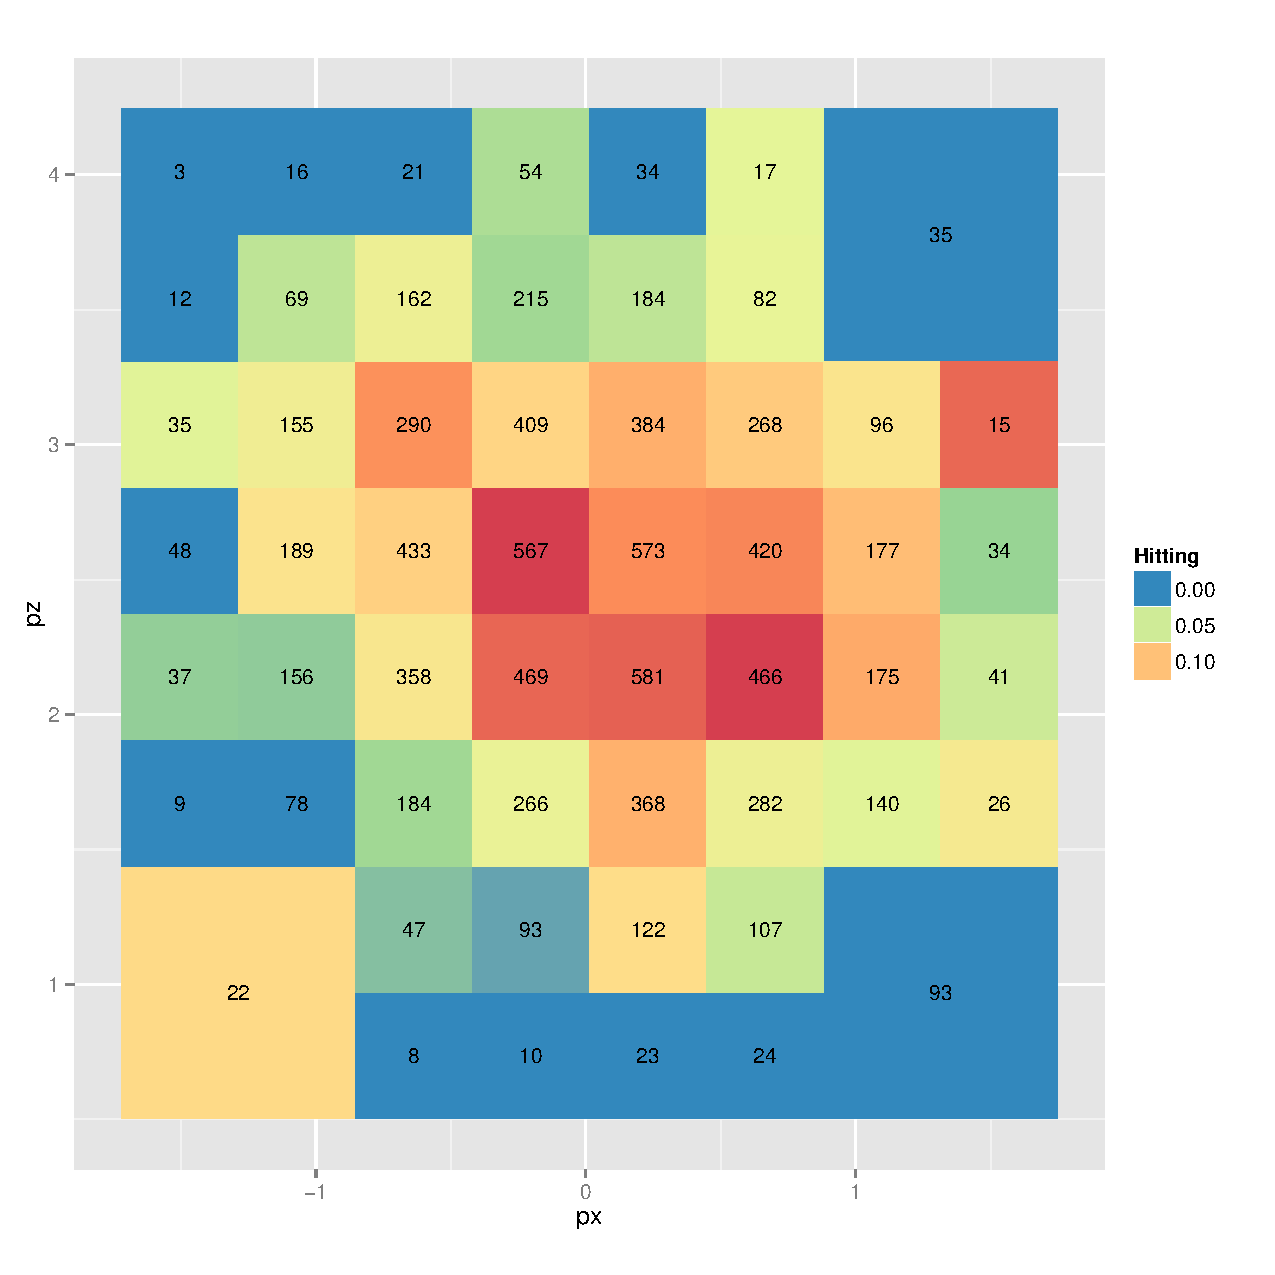
\includegraphics[scale=.2]{Images/Chapter8x8_100.pdf}
      	\caption{...(these images, and others, need labels: (A) (B) (C) etc)}
\end{figure} 
For this reason the bottom left heat maps in Figures 7 and 8, shown in Figure 9, differ in the number of boxes of each size, and the total number of boxes. This divergence continues at the next iteration, where the stopping rule $n_{b} < 100$ requires 28 box subdivisions in Figure 8, map three; and $n_{b} < 200$ gives 16 box subdivisions in Figure 7, map three.

% *Alix: ``I wonder if there's any literature on the physics from a hitter's perspective in terms of how small a difference in location is even detectable.

% *Alix: ``Great start Chris. --> need to add more about how one would now interpret the ``best'' empirical heat map.

\subsection{Heat Map Confidence Intervals with Shiny}

% =========================
\section{Generalized Linear Models for Hitter Success Probabilities} 

Our goal is to create a statistical model for the heat map of success probabilities. Nonparametric methods, while straightforward, sacrifice interpretability; while they achieve a modeled heat map, there may not be interpretable components of the model. Nonparametric models cannot relate spatially varying hitter success probabilities to hitter attributes. We propose a parametric approach using biomechanically interpretable covariates. Existing research analyzes the biomechanics of the baseball swing \citep{Welch1995}, but no research integrates those results with spatial swing outcomes in a statistical model.


Let success indicator variable, $Y_{ijklm}$, be a Bernoulli random variable with spatially varying mean \citep{Ross2002}. Subscript $i = 1, \dots, n_{jklm}$ indexes hitter $j$'s swings in at bat $k$ against pitcher $l$ in year $m$. Subscript $k = 1, \dots, n_{jlm}$ indexes hitter $j$'s at bats against pitcher $l$ in year $m$. Subscript $l = 1, \dots, n_{jm}$ indexes pitchers hitter $j$ faced, where $n_{jm}$ is the total number of pitchers hitter $j$ faced; and $m = 2007, \dots, 2016$ indexes year. Let $\pmb{s}_{ijkl} = (px_{ikl}, pz_{ijkl})\in \pmb{D} \subseteq \pmb{R}^{2}$ be the horizontal and vertical locations, respectively, of pitch $ijkl$ as it passes through the two dimensioned vertical face of the hitting zone. The origin, $\pmb{s}_{\cdot} = (0,0)$, is the midpoint of the front edge of home plate, at ground level. From the pitcher's point of view, pitches to the left (right) of the center of home plate correspond to negative (positive) values of $px_{\cdot}$. Pitches that bounce before reaching home plate correspond to negative values of $pz_{\cdot}$.  

In this study we make the simplifying assumption that location success probabilities depend on only location and hitter. This means we dispense with subscripts $k, l,$ and $m$. We also assume that, given pitch location to hitter $j$, $\pmb{s}_{ij} = (px_{ij}, pz_{ij})$,  swings are independent Bernoulli trials. This gives $Y_{ij}|\pmb{s}_{ij} \sim \text{Bernoulli}(p_{ij})$, where $\text{E}[Y_{i}|\pmb{s}_{ij}] = p_{ij}$

Accordingly, let $i = 1, \dots, n_{j}$ index hitter $j$'s swings, out of $n_{j}$ total swings on record. Let $\pmb{X}_{ij}(\pmb{s}_{i})$ be covariates specific to hitter $j$ and location $\pmb{s}_{ij}$ on swing $i$. A Bernoulli random variable suggests a generalized linear model with logit link function for relating success probability to covariate information: 

\begin{equation}
\text{logit}(p_{ij}|\pmb{X}_{ij}(\pmb{s}_{ij})) = \pmb{X}_{ij}(\pmb{s}_{ij}) \pmb{\beta}_{j},
\end{equation}

where $\pmb{\beta}_{j}$ is the vector of covariate coefficient parameters specific to hitter $j$ \citep{Myers2012}. Next, we discuss and develop covariates.

\subsection{Biomechanically Interpretable Covariates} % ==============

Why does Peralta, and why do hitters in general, hit pitches in some locations better than others? We submit biomechanics as potentially part of the answer. Biomechanics underpin why hitters prefer some pitch locations more than others. Given the choice, athletes select a specific place for the ball before swinging. Consider golf, a sport where the ball is stationary, and the acting athlete chooses where to stand in relation to the ball. In fact, golfers position themselves very precisely in relation to the ball to achieve impact at the optimal point in their swing \citep{Cochran2005}. If the impact point deviates from the ideal location, performance suffers. Consider tennis, a step closer to baseball, in that the ball approaches, but the player has time to position himself relative to the incoming ball. Once again, tennis players strive to hit the ball at a specific point in their forehand, a precise distance from the ground and from their body \citep{Elliott2006}. As with golf, if the point of impact deviates from this location, performance suffers. Note that in both sports the ideal player to ball positioning depends on, at the very least, anatomy, biomechanics, and equipment. We submit the same dynamics affect baseball hitting. However, in baseball the hitter cannot predtermine ball location, nor does he have time to reposition himself in response to the location and trajectory of the incoming pitch. For these reasons, meaningful measurements of hitter to ball distance and angle are reasonable covariates. Polar coordinate pitch locations would inherently provide this type of meaningful covariate for use and interpretation in our models. 

To illustrate, in Figure 3 we shift the origin to a hitter's approximate center of gravity in his stance, where the extended bat line intersects his axis of rotation at the moment of contact \citep{Welch1995}. 

% \footnote{We will determine the translated origin location based on additional biomechanics research, in consultation with two baseball biomechanics research directors. See the final two paragraphs of this section for details.}.  

  \begin{figure}[H]
	\centering
	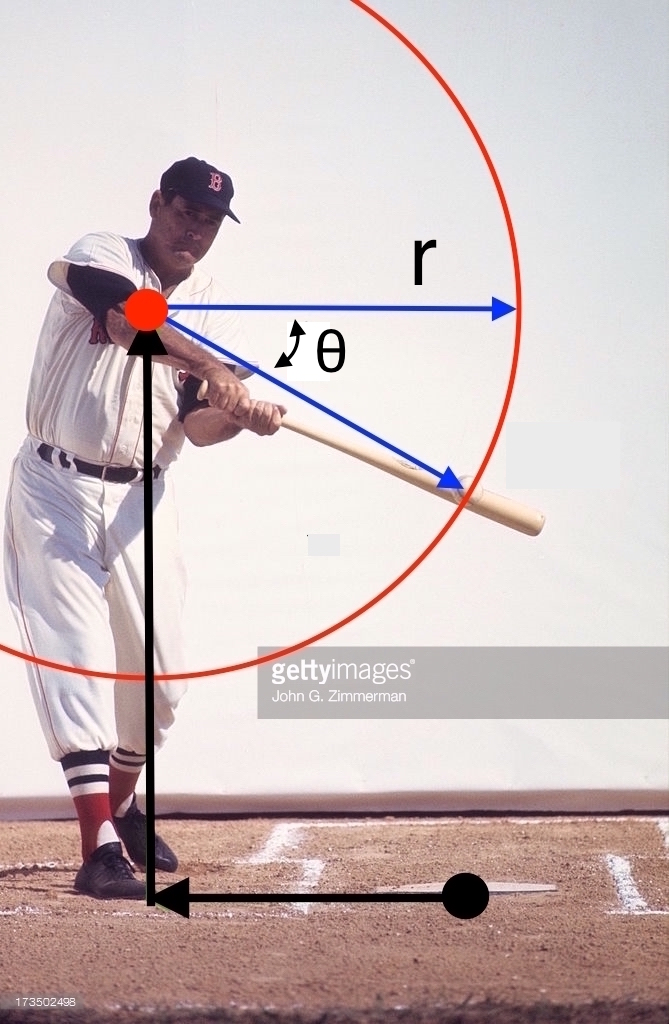
\includegraphics[scale=.15]{Images/WilliamsPolar.jpg} 
	\caption{The ground level black dot represents the origin (0,0) in the rectangular coordinate system. The translated origin (red dot) coincides with the hitter's approximate center of gravity, and thus the polar origin. The bold arrows show the origin shift. The length of the arrows moving out from his center of gravity to specific grid locations represent $r$, and the angle between the same two arrows represent $\theta$.}
	\end{figure} 
Referring to Figure 3, let $r$ measure the distance from the hitter's center of gravity to the ball at impact, and let $\theta$ be the angle below horizontal of the line segment connecting the center of gravity and the ball at impact. As in golf and tennis, ball location---too far/close to the hitter, or above/below the ideal point of impact--- affects hitting performance. Letting $\pmb{X}_{ij}(\pmb{s}_{ij})$ in (1) be comprised of $r_{ij}$ and $\theta_{ij}$ terms provides an exploratory starting point.

% ===== ======= ====== ====== ===== ====== ====== ======
\subsection{Generalized Linear Model with Biomechanically Interpretable Covariates} 

Let covariate vector $\pmb{X}_{ij}(\pmb{s}_{ij})$ in (1) be defined as $\pmb{X}_{ij}(\pmb{s}_{ij}) = \{r_{ij}, \theta_{ij}, r_{ij}\theta_{ij}, r_{ij}^{2}, \theta_{ij}^{2}, r_{ij}^{2}\theta_{ij}^{2}\}$. Substituting into (1) yields:
\begin{equation}
\text{logit}(p_{ij}|\pmb{s}_{ij}, r_{ij}, \theta_{ij}) = \beta_{j0} + \beta_{j1}r_{ij} + \beta_{j2} \theta_{ij} + \beta_{j3} r_{ij} \theta_{ij} + \beta_{j4}r_{ij}^{2} + \beta_{j5} \theta_{ij}^{2} + \beta_{j6} r_{ij}^{2} \theta_{ij}^{2}
\end{equation}

Note that given a hitter $j$, and pitch location $\pmb{s}_{ij}$, the elements of $\pmb{X}_{ij}$ are simply a trigonemtric function of $\pmb{s}_{ij}$ and the translated origin. Thus, for convenience, we replace $\text{logit}(p_{ij}|\pmb{s}_{ij}, r_{ij}, \theta_{ij})$ with $\text{logit}(p_{ij}|\pmb{s}_{ij})$ for the remainder of this study.

We choose Johnny Peralta from Chapter 1 to illustrate, and let $j = P$ for convenience. We fit model (2) using Peralta's $n_{P} = 9177$ observed swings, find maximum likelihood estimates of $\pmb{\beta}_{P}$ using an iteratively reweighted least squares algorithm \citep{Myers2012}. 

(IT WOULD BE NICE: EMPIRICAL, ESTIMATES, FITTTED HEAT MAP) \\
% \centering
\begin{tabular}{ l | c | c | c | r }

    \hline
    Covariate         & Parameter   & MLE   & SE     &      p    \\ \hline \hline
    N/A               & $\beta_{0}$ & -4.08 & 0.70 & $ <0.001$ \\ \hline
    r                 & $\beta_{1}$ &  1.19 & 0.51 & $  0.018$ \\ \hline
    $\theta$          & $\beta_{2}$ & -1.93 & 1.90 & $  0.311$ \\ \hline
    $r*\theta$        & $\beta_{3}$ & -1.64 & 0.70 & $  0.064$ \\ \hline
    $r^{2}$           & $\beta_{4}$ & -0.32 & 0.09 & $ <0.001$ \\ \hline
    $\theta^{2}$      & $\beta_{5}$ & -3.92 & 1.10 & $ <0.001$ \\ \hline
    $r^{2}*\theta^{2}$& $\beta_{6}$ & -0.46 & 0.21 & $  0.025$ \\ \hline
    \hline  

  \end{tabular}

  \begin{figure}[H]
  % \centering
	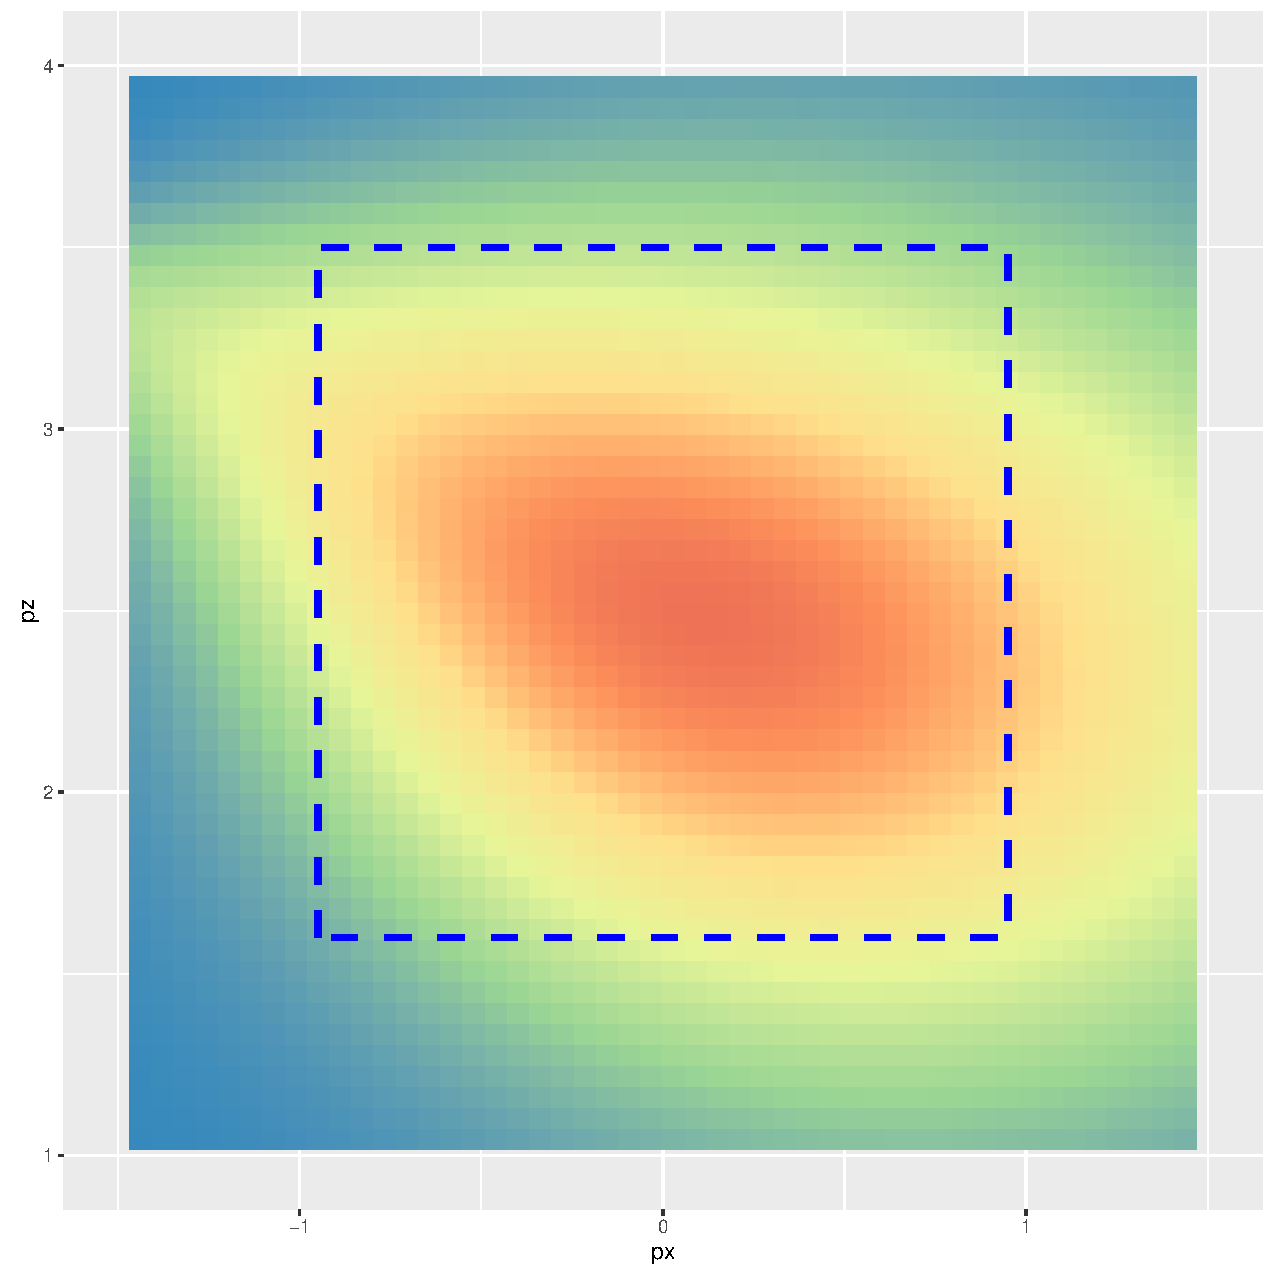
\includegraphics[scale=.3]{Images/Peralta_polar.pdf} 
  \caption{}
  
	\end{figure} 

\subsection{Hosmer-Lemeshow Goodness of Fit Test} % ================

Generalized Linear Models \citep{Myers2012}

  \begin{itemize} % ===============
  \item (pg 147) Hosmer-Lemeshow test = Logistic regression Goodness of Fit test. 
  \item Like Pearson Chi-Sq, but for continuous covariates. 
  \item Order all responses according to fitted $\hat{p}$, then group into deciles. 
  \item Then basically $\chi^{2} = \Sigma \Sigma \frac{(O - E)^{2}}{E}$
  \item p-value = 0.1513
  \end{itemize}

% ================== 
\section{Spatial Generalized Linear Mixed Models for Hitter Success Probabilities}

\subsection{Introduction} % ================== 

No matter the performace of the previously fit model, we expect there to be unexplained spatial variation in the mean. The covariates are limited in scope and depth, and Tobler's First Law of Geography tells us that things close together in space tend to behave more similarly than things further apart \citep{Tobler1970}. Accordingly, we enhance the model to capture the unexplained spatial variation in the mean, and compensate for unobserved covariates, by adding a spatially correlated random effect  \citep{Banerjee2008}. 

\subsection{Gaussian Random Field} % ================== 

A Gaussian random field is a popular and practical distribution for spatial random effects \citep{Gelfand2010}. Let random variable vector $\pmb{w}(\pmb{s})$, for vector of locations $\pmb{s} \in \pmb{D} \subseteq \pmb{R}^{2}$, be distributed multivariate Normal with mean $\pmb{0}$; with symmetric, positive definite covariance matrix $\Sigma(\pmb{\theta})$, and covariance parameter vector $\pmb{\theta}$ \citep{Haran2011}.
\begin{equation}
\pmb{w} | \pmb{\theta} \sim MVN(\pmb{0}, \Sigma(\pmb{\theta})) 
\end{equation}

Including a random effect defined in this way, with a valid covariance matrix, would retool (2) as a {\it spatial} generlatized linear {\it mixed} model (SGLMM). Next we define the covariance structure we use in this study.

\subsection{Exponential Covariance}
To add a spatial random effect, distributed as a Gaussian random field, to the linear predictor in (2), it remains to define a spatial correlation structure to $\pmb{w}$. Let $w_{ij}$ be defined as in {\bf 5.1}, with an exponential covariance structure. That is, the i,jth element of $\Sigma(\phi, \sigma^{2})$ is:
\begin{equation}
\Sigma(\phi, \sigma^{2})_{i,j} = \sigma^{2} exp(-||\pmb{s}_{i} - \pmb{s}_{j}||/\phi),
\end{equation}
where $||s_{i} - s_{j}||$ is the Euclidean distance between $\pmb{s}_{i}$ and $\pmb{s}_{j}$, $\sigma^{2}$ is the scale parameter, and $\phi$ is the range parameter.

\subsection{Spatial Generalized Linear Mixed Model}
Inserting $\pmb{w}(\pmb{s})$ to the linear predictor in (1) gives the following spatial generalized linear mixed model (SGLMM):
\begin{equation}
\text{logit}(p_{ij}|\pmb{s}_{ij}) = \pmb{X}_{ij}(\pmb{s}_{ij}) \pmb{\beta}_{j} + w(\pmb{s}_{ij}).
\end{equation}

This spatial hierarchical model, with its latent Gaussian random field, gives $p_{ij}$ a complicated correlation structure. Bayesian statistical methodologies, primarily Markov chain Monte Carlo (MCMC) methods, are very popular for fitting spatial models of this kind \citep{Banerjee2014}. In fact, MCMC is one of the few practical approaches available to fit a `big n' model with complex spatial correlation. This is because of the `big n problem' \citep{Lindgren2011}. Namely, the computational costs for SGLMMs increase at a rate of $\mathcal{O}(n^{3})$ (REFERENCE). This rate of increase leads to prohibitively slow model fitting. To attempt to fit SGLMMs in practically useful time spans, we try: 

To estimate model parameters for (4) we tried:
\begin{enumerate}
\item Computational optimization, C++, an efficient algorithm, with Hamiltonian Monte Carlo in Stan
\item Dimension reduction with Predictive process models in \verb|spBayes|
\item INLA SPDEs and \verb|INLA-R|
\end{enumerate}

Note that the ultimate goal of this research is practical, real-time applications for baseball fans, broadcasts, players, scouts, and teams. Therefore, model fitting speed matters on a finer time scale than academic research demands.  

\subsection{Markov Chains}

Hierarchical Modeling and Analysis for Spatial Data \citep{Banerjee2014}
        \begin{itemize} % ===============
        \item ``Without doubt, the most popular computing tools in Bayesian practice today are Markov chain Monte Carlo (MCMC) methods.'' 
        \item inference from posteriors of ``...arbitrarily large dimension, essentially by reducing the problem to one of recursively solving a series of lower-dimensional (often unidimensional) problems.'' 
        \item ``...work by producing not a closed form for posterior, but a sample of values $\{\theta^{(g)}, g = 1, \dots, G\}$ from this distribution.'' ($G$ = number of draws from posterior) 
        \item Two issues: MCMC algorithms produce {\it correlated} draws from poster (hence thinning, acf(), pacf(), and {\it convergence} diagnosis 
        \item Two most popular MCMC algorithms: (1) Gibbs sampler (2) Metropolis Hastings algorithm
        \end{itemize} % ===============
        
\section{Method 1 - HMC in Stan} % =================

\subsection{Hamiltonian Dynamics and MCMC} % =================

\footnote{The history and physics presented in this section owe heavily to, and are primarily informed by, \citep{Neal2011}} Trying to understand molecular states, \cite{Metropolis1953} created MCMC for ``fast machines.'' Later, modeling molecular motion as a deterministic process, \cite{Alder1959} introduced {\it Hamiltonian dynamics} as an alternate representation of Newtonian mechanics. Almost 30 years later, \cite{Duane1987} combined the two to create ``hybrid Monte Carlo'' to simulate certain quantum mechanical processes. Over time, this named morphed into {\it Hamilton} Monte Carlo (HMC), as it is known today. Eventually, \cite{Neal1996} used HMC methods for explicitly statistical applications, studying neural networks.

HMC works by reframing the variables and distribution of interest as part of a physical system. From a physics standpoint, an object in a well defined three dimensional physical space can be completely characterized by its position and momemtum. For HMC, the variables of interest function as position variables, and auxiliary Gaussian variables are introduced serve as momentum variables. Simple updates for the auxiliary momentum variables generate, via a system of differential equations, proposals for Metropolis updates to the more important position variables (which represent the variabls of interest). The differential equation solutions estimate trajectories of the hypothetical physical object, which will then occupy a new position after some chosen time step. This crafty formulation enables distant, yet high probability, proposals for the variables of interest. Note that this contrasts favorably, in terms of mixing, to the random walk proposal generation process commonly used for Metropolis updates.

\subsection{Hamilton Equations for MCMC} % =================

Let $q(t)$ be a d-dimensional ($d$ parameters of interest) position vector that is a function of time $t$; and $U(q(t))$ represent the potential energy at time $t$. Let $p(t)$ give the d-dimensional momentum at time $t$, and $K(p(t))$ represent kinetic energy at time $t$. Then the Hamilton equation,
\begin{equation}
H(q(t),p(t)) = U(q(t)) + K(p(t)),
\end{equation}
measures the total energy of a system. 

For HMC applications, we let the potential energy, $U(q)$, be minus the log of the probability density function of interest, plus any convenient constant\footnote{We omit $t$ for clarity of presentation, here and elsewhere, but position and momentum remain functions of time $t$.}. Typically, HMC procedures define $p$ as a d-dimensional zero mean Gaussian with covariance matrix M, and $K(p)$ as minus the log of the multivariate Gaussian probability density function. This gives:
\begin{align}
H(q,p) = -\text{log}f_{q}(q) + p^{T}\pmb{M}^{-1}p/2.
\end{align}

This clever formulation provides useful partial derivatives for calculating the change in position and momentum over time. For $i = 1,\dots, d$:
\begin{align}
\frac{d q_{i}(t)}{dt} &= \frac{\partial H}{\partial p_{i}}, \\
\frac{d p_{i}(t)}{dt} &= -\frac{\partial H}{\partial q_{i}}.
\end{align}
Substituting in Hamilton's equation (5) and simplifying gives
\begin{align}
\frac{d q_{i}(t)}{dt} &=  [\pmb{M}^{-1}p]_{i} \\
\frac{d p_{i}(t)}{dt} &= \frac {\partial \left[ \text{log}f_{q}(q) \right]}{\partial q_{i}}
\end{align}
The solutions to these two differential equations, that is $q(t)$ and p(t) such that (8) and (9) hold, give the instantaneous rate of change of position and momentum at time t. 

subsection{MCMC Using Hamiltonian Dynamics \citep{Neal2011}} % =================
Steps.

\begin{itemize}

\item {\bf Leapfrog method} = for calculating new position (q) and momentum (p) through tiny time steps
  \begin{itemize}
  \item for {\bf discretizing Hamilton equations}
  \item akin to Taylor Series appoximations
  \item Postion (q) (or momentum (p)) at $t_{0}$ plus time step times rate of change of position (q) (momentum (p)) variable at $t_{0}$
  \item Leapfrom Method does half step for momentum (p), full step for postion (q), other half step for momentum (p). Damn good.

  \end{itemize}

\item Short version: randomly sample from K(p) (kinetic, momentum), calculate U(k) (potential, position*) --- that's your Metropolis proposal.
\end{itemize}


\subsection{Optimizing in Stan} % =================
`Big n' computational burdens can also be mitigated somewhat, by certain program specific coding techniques. These techniques, as well as other techniques aimed to encourage model convergence, bolstered our modelling efforts. We highlight some such techniques for Stan here, and include the complete .stan script in Appendix A for reference. 

\subsubsection{Bayesian Motivated Techniques} % =================

Stan allows a user to omit prior distributions for parameters, but interprets non-inclusion as a non-informative, uniform prior. However, \cite{Gelman}, the first Stan developer, pointed out in correspondence that the exponential covariance length-scale parameter, $\phi$ in equation (3), requires an informative prior for model identifiability (CITATION?). \cite{Trangucci} recommended, in particular, a sharp tailed prior distribution for the length-scale parameter, such as the normal or log-normal, to act as soft upper and lower bound constraints\footnote{``Without stronger priors on l, GP can act as a second constant term in your regression for large draws of length-scale and large draws of alpha.''}. Even further, for practical computing time and convergence considerations, \cite{Trangucci} said complex models such as spatial hierarchical models require proper priors for all $\beta$ coefficients. Using the intial GLM estimates to inform coefficient prior distributions had exactly the intended effects.

\subsubsection{Computational and Linear Algebra Motivated Techniques} % =================
For speed and efficiency, the Stan Users Manual recommends pure matrix algebra and vectors, over `for loops' and scalars \cite{StantheMAN}. For example, 
\begin{verbatim}
hit ~ bernoulli_logit(X*beta + Z)
\end{verbatim}
is faster than
\begin{verbatim}
for (n in 1:N)
        hit[n] = bernoulli_logit(X[n]*beta[n] + Z[n]);
\end{verbatim}
Notice that $N \times 1$ column vectors \verb|hit|, \verb|beta|, and \verb|Z| replace scalars \verb|hit[n]|, \verb|beta[n]|, and \verb|Z[n]|; and $N \times p$ matix \verb|X| replaces $1 \times p$ row vector \verb|X[n]|.

\cite{Trangucci} also suggested a QR factorization on covariate matrix $\pmb{X}$, in the linear predictor, to increase computational efficiency. A QR factorization consists of factoring an $n \times p$ matrix into the product of an $n \times p$ orthogonal matrix $\pmb{Q}$ and a $p \times p$ upper triangular matrix $\pmb{R}$, such that $\pmb{X} = \pmb{QR}$. 
\begin{align}
\pmb{X} &= \pmb{QR} \\
\pmb{X \beta} &= \pmb{QR \beta}
\end{align}
To reparameterize for model fitting, let $\pmb{\theta} = \pmb{R \beta}$, so that $\pmb{\beta} = \pmb{R^{-1}\theta}$, which gives
\begin{align}
\pmb{X \beta} &= \pmb{Q \theta}, \text{ and } \\
\text{logit}(p_{ij}|\pmb{s}_{ij}) &= \pmb{Q}_{ij}(\pmb{s}_{ij}) \pmb{\theta}_{j} + w_{ij}.
\end{align}
Now prior information about $\pmb{\beta}$ should be incorporated into and given in the prior distributions of $\pmb{\theta}$. Consider non-informative prior distributions on $p$ dimensional parameter vector $\pmb{\beta}$,
$$ \pmb{\beta} \sim N(\pmb{0}, \sigma^{2}\pmb{I}_{p}), $$
where $\pmb{I}_{p}$ is the $p \times p$ identity matrix, and $\pmb{0}$ is a $p \times 1$ zero vector. Notice the intended variance of the non-informative prior must be modified for $\pmb{\theta}$.
\begin{align}
\text{Var}(\pmb{\theta}) &= \text{Var}(\pmb{R \beta}) \\
&= \pmb{R}\text{Var}(\pmb{\beta})\pmb{R}' \\
&= \pmb{R}\sigma^{2}\pmb{I}_{p}\pmb{R}' \\
&= \sigma^{2} \pmb{R}\pmb{R}'
\end{align}

We add noise to the covariance matrix diagonal with the following snippet of code.
\begin{verbatim}
for (n in 1:N)
  Sigma[n, n] = Sigma[n, n] + 1e-6;
\end{verbatim}
This added diagonal noise guarantees that the covariance matrix assembled by \verb|cov_exp_quad(...)| remains numerically positive-definite \cite{Trangucci2017}. This \verb|cov_exp_quad(...)| function can generate numerically non-positive-definite matrices when operating at high dimensions.

Finally, \cite{Carpenter} recommended a Cholesky decomposition and tactical reparameterization, noting the efficiency of a vectorized scalar approach.
\begin{verbatim}
L = cholesky_decompose(Sigma);  
Z ~ normal(0, 1);  
Z_mod = L * Z; 
hit ~ bernoulli_logit(Q*theta + Z_mod);
\end{verbatim}
The first line performs a Cholesky decomposition on the covariance matrix \verb|Sigma|. A Cholesky decomposition factors symmetric matrix \verb|Sigma| such that $\Sigma = \text{\pmb{LL}}'$. The second, ``vectorized scalar'' line generates $n$ standard normal random variables, by reusing \verb|normal(0, 1)| for every element of \verb|Z|. These two lines remove the dependence of random vector \pmb{Z}, which must be generated, on unknown parameters to be estimated \cite{Trangucci2017}. The third line transforms \verb|Z| to have the desired distribution. Note that $\text{Var}(\text{\pmb{LZ}}) = \text{\pmb{L}} \text{I}_{n}\text{\pmb{L}}' = \Sigma$, so that $\pmb{LZ} \sim N(\pmb{0}, \Sigma)$ as desired.

\subsection{``Big N Problem''}

\subsubsection{Evaluate Inverse you say?? Yes.}


\begin{itemize}
\item logit\{EY(s)\} = $\pmb{X}(s)\pmb{\beta} + Z(s)$, with $Z(s) \sim MVN\{\pmb{0}, \Sigma_{s}\}$
\item $f(\pmb{\beta}, \phi, \sigma^{2}, \pmb{Z}|\pmb{Y}) \propto f(\pmb{Y}|\pmb{\beta}, \phi, \sigma^{2}, \pmb{Z})f(\pmb{\beta})f(\pmb{Z}|\phi, \sigma^{2})f(\phi)f(\sigma^{2})$
\item M-H proposal, iteration i: $Z_{10,i}$
$$ r = \frac{ f(Z_{10,i}|\pmb{Z}_{1:9,i},\pmb{Z}_{11:n,i-1}, \pmb{\beta}_{i-1}, \phi_{i}, \sigma^{2}_{i})}{f(Z_{10,i-1}|\pmb{Z}_{1:9,i},\pmb{Z}_{11:n,i-1}, \pmb{\beta}_{i-1}, \phi_{i}, \sigma^{2}_{i})} $$
 
\item Note: $f(z_{1}, z_{2}, z_{3}|\pmb{Y}) = f(z_{1}|z_{2},z_{3},\pmb{Y})f(z_{2},z_{3}|\pmb{Y})$. So... $$r \propto \frac{f(\pmb{Y}|\pmb{\theta}_{i})f(\pmb{\beta})f(Z_{10,i}|\pmb{Z}_{1:9,i},\pmb{Z}_{11:n,i-1}, \phi_{i}, \sigma^{2}_{i})f(\pmb{Z}_{1:9,i},\pmb{Z}_{11:n,i-1}|\phi_{i}, \sigma^{2}_{i})f(\phi)f(\sigma^{2})} {f(\pmb{Y}|\pmb{\theta}_{i-1})f(\pmb{\beta})f(Z_{10,i-1}|\pmb{Z}_{1:9,i},\pmb{Z}_{11:n,i-1}, \phi_{i}, \sigma^{2}_{i})f(\pmb{Z}_{1:9,i},\pmb{Z}_{11:n,i-1}|\phi_{i}, \sigma^{2}_{i})f(\phi)f(\sigma^{2})}$$

$$ r \propto \frac{f(\pmb{Y}|\pmb{\theta}_{i})f(Z_{10,i}|\pmb{Z}_{1:9,i},\pmb{Z}_{11:n,i-1}, \phi_{i}, \sigma^{2}_{i})}
{f(\pmb{Y}|\pmb{\theta}_{i-1})f(Z_{10,i-1}|\pmb{Z}_{1:9,i},\pmb{Z}_{11:n,i-1}, \phi_{i}, \sigma^{2}_{i})} $$

\item And $f(\pmb{Z})$, $f(Z_{i}|\pmb{Z}_{-i})$, etc. are $MVN\{\cdot,\Sigma^{*}\}$, where $\Sigma^{*}$ either is, or is some function of, $\Sigma_{\pmb{s}}$; with PDF kernal containing $\Sigma_{\pmb{s}}^{*-1}$, (containing $\phi_{i}, \sigma^{2}_{i})$.

\end{itemize}

\section{Method 2 - Predictive Process Models in spBayes} % =========

Predictive process models (PPMs) provide a method for attempting to circumvent the ``big N problem'' in the case of Bayesian hierarchical models with latent Gaussian random effects. Numerous methods exist, for example \citep{Cressie2008}, (CITE OTHERS), but predictive process models provide a competitive modeling approach with computational advantages for hierarchical models with a Gaussian random field (GRF) at the second level of specification \citep{Banerjee2008}. Latent GRFs prove challenging because they are only implicitly observed, through a binomial response in our case. This means the GRF parameters (hyperparameters) and their prior distributions comprise the third level of the hierarchical model. Gaussian PPMs achieve dimension reduction by projecting the original process onto a lower dimensioned subspace, at a set of locations called knots \citep{Banerjee2008}. 

\subsection{PPM Procedure}

Consider again the SGLMM (5), and Gaussian random field $\pmb{w}(\pmb{s})$.
\begin{align}
\text{logit}(p_{ij}|\pmb{s}_{ij}) &= \pmb{X}_{ij}(s_{ij}) \pmb{\beta}_{j} + w(\pmb{s}_{ij}) \\
\pmb{w}(\pmb{s}) | \pmb{\theta} &\sim \text{GRF}(\pmb{0}, \pmb{C}(\pmb{\theta}))
\end{align}

Define (20) as in (5), and (21) shows $n \times 1$ vector of random effects $\pmb{w}$ at locations $\pmb{s}$, conditioned on covariance parameters $\pmb{\theta}$, constitutes a GRF. Let $n \times 1$ zero vector $\pmb{0}$ be the stationary GRF mean, with $n \times n$, symmetric, positive-definite covariance matrix $\pmb{C}(\pmb{\theta})$. Let $C(\pmb{s}_{i}, \pmb{s}_{j}; \pmb{\theta})$ denote the covariance of random effects at locations $\pmb{s}_{i}$ and $\pmb{s}_{j}$, so that $C(\pmb{\theta}) = [C(\pmb{s}_{i}, \pmb{s}_{j}; \pmb{\theta})]_{i,j=1}^{n}$.

To define the PPM, start with knot locations. Let $\pmb{S}^{*} = \{\pmb{s}_{1}^{*}, \dots, \pmb{s}_{m}^{*}\}$ be a set of $m < n$ chosen knot locations, which may or may not be a subset of observed locations. We denote knot location random effects with $m \times 1$ vector $\pmb{w}^{*} = \left[w(\pmb{s}_{i}^{*})\right]_{i=1}^{m}$, and the $m \times m$ knot covariance matrix and its elements as $\pmb{C}^{*}(\pmb{\theta}) = \left[C(\pmb{s}_{i}^{*}, \pmb{s}_{j}^{*})\right]_{i,j = 1}^{m}$. The knot random effects form a distinct $m$-dimensional GRF.
\begin{equation}
\pmb{w}^{*}|\pmb{\theta} \sim \text{GRF}\{\pmb{0}, \pmb{C}^{*}(\pmb{\theta})\}
\end{equation}
The predictive process modelling procedure uses the $m$ selected knots, the covariance structure of the parent process, and kriging to interpolate $w$ at site $\pmb{s}_{0}$ \citep{Schabenberger2004}; See Appendix ?? for kriging details. Let $\tilde{w}(\pmb{s}_{0})$ represent this interpolated random effect, and let $\pmb{c}(\pmb{s}_{0};\pmb{\theta}) = \left[C(\pmb{s}_{0}, \pmb{s}_{j}^{*}; \pmb{\theta})\right]_{j = 1}^{m}$ be an $m \times 1$  covariance vector giving the covariance of the $\pmb{s}_{0}$ random effect with the knot random effects.
\begin{align}
\tilde{w}(\pmb{s}_{0}) &= E[w(\pmb{s}_{0})|\pmb{w}^{*}] \\ 
&= \pmb{c}^{T}(\pmb{s}_{0};\pmb{\theta}) \cdot \pmb{C}^{*-1}(\pmb{\theta}) \cdot \pmb{w}^{*}
\end{align}
For a GRF, the weights of linear combination (24) minimize the squared error loss function among all linear predictors \citep{Schabenberger2004}; and notice that the linear combination varies spatially. Accordingly, predictive process $\tilde{w}(\pmb{s})$ defines another GRF and covariance matrix.
\begin{align}
\tilde{\pmb{w}}(\pmb{s}) &\sim \text{GRF}\{0, \tilde{C}(\cdot)\} \\
\tilde{C}(\pmb{s}, \pmb{s}'; \pmb{\theta}) &= \pmb{c}^{T}(\pmb{s};\pmb{\theta}) \cdot \pmb{C}^{*-1}(\pmb{\theta}) \cdot \pmb{c}(\pmb{s}';\pmb{\theta})
\end{align}
To reiterate, $m \times 1$ vector $\pmb{c}(\pmb{s};\pmb{\theta}) = \left[C(\pmb{s}, \pmb{s}_{j}^{*})\right]_{j = 1}^{m}$ gives the covariance of the random effect at $\pmb{s}$ with knot random effects. Finally, the predictive process model:

\begin{equation}
\text{logit}(p_{ij}|\pmb{s}_{ij}) = \pmb{X}_{ij}(\pmb{s}_{ij}) \pmb{\beta}_{j} + \tilde{w}(\pmb{s})
\end{equation}




\subsection{Improved Predictive Process Models}

\subsection{Predictive Process Models in spBayes}




\section{Method 3 - INLA and SPDEs} % =================

\subsection{Gaussian Markov Random Fields}

\subsection{Integrated Nested Laplace Approximations (INLA)}

\subsection{Stochastic Partial Differential Equations (SPDE)}

\subsubsection{Stochastic Calculus}

\subection{Bayesian Inference with INLA and SPDEs}

\appendix
\section{Stan Code for Hamiltonian MCMC} % =================
\begin{verbatim}
data {                             
  int<lower=0> N;                 // N observations
  int<lower=0> p;                 // p predictors
  matrix[N,p] Q;                  // QR decomp - Q
  matrix[p,p] R;                  // QR decomp - R
  int<lower=0, upper=1> hit[N];   // 0/1 outcomes; array of integers
  vector[2] px_pz[N];             // N-dim array of 2-dim vectors
  vector[p] theta_SDs;            // theta prior SDs
}
transformed data{
  matrix[p,p] R_inv;
  R_inv = inverse(R);
}
parameters {                
  real<lower=0> l;                  // length-scale parameter
  real<lower = 0> sigma;            // scale parameter
  real beta0;                       // intercept 
  vector[p] theta;
  vector[N] Z;                      // location random effect
}
transformed parameters {
      vector[p] beta;
      beta = R_inv*theta;
}
model {  
  matrix[N, N] Sigma;
  matrix[N, N] L;                     // Lwr triangular Cholesky decomp
  vector[N] Z_mod;
      
      l ~ lognormal(-2,1);            // E[l] = 0.223
      sigma ~ lognormal(-1.5, 1.5);   // E[sigma] = 0.687
      beta0 ~ normal(0,5);
      
      theta[1] ~ normal(0, theta_SDs[1]);
      theta[2] ~ normal(0, theta_SDs[2]);
      theta[3] ~ normal(0, theta_SDs[3]);
      theta[4] ~ normal(0, theta_SDs[4]);
      theta[5] ~ normal(0, theta_SDs[5]);
      theta[6] ~ normal(0, theta_SDs[6]);
      
      Sigma = cov_exp_quad(px_pz, sigma, l); 
      for (n in 1:N)
        Sigma[n, n] = Sigma[n, n] + 1e-6;
      L = cholesky_decompose(Sigma); // Sigma = LL' 
      
      Z ~ normal(0, 1);  // Each element is N(0,1)
      Z_mod = L * Z; // (Cov matrix Cholesky)*MVN(0,1)
      
      hit ~ bernoulli_logit(beta0 + Q*theta + Z_mod);
}
\end{verbatim}

\section{R Code, spBayes for Predictive Process Models} % =================

\section{R Code, R-INLA for INLA}
% To facilitate explanation, let location $ij$ vector $\pmb{s}_{ij}$ now be denoted $s_{ij}$, keeping in mind that $s_{ij}$ is still a two-dimensioned vector. Instead, let $\pmb{s}$ denote the $n \times 1$ vector of all locations where we observed a $Y_{ij}$. 

\section{Kriging}

From: ``Statistical Methods for Spatial Data Analysis'' \citep{Schabenberger2004}

The mean is known---Simple Kriging
\begin{enumerate}
\item Spatial data: $\mathbf{Z(s)} = [Z(s_{1}), Z(s_{2}),\hdots, Z(s_{n})]'$

\item Assume: $\mathbf{Z(s) = \mu(s) + e(s)}$, $\mathbf{e(s) \sim (0, \Sigma)}$, where $\mathbf{0, \Sigma}$ known.

\item Goal: find predictor $p(\mathbf{Z};s_{0})$, of $Z(s_{0})$, that minimizes $E\left[ \left(p(\mathbf{Z};s_{0}) - Z(s_{0}) \right)^{2}\right]$ 

\item Consider only linear predictors of the form: $p(\mathbf{Z};s_{0}) = \lambda_{0} + \mathbf{\lambda 'Z(s)}$

\item Expand, simplify, set derivative equal to zero.

\item Note: Var$[Z(s_{0})] = \sigma^{2}$, and $\mathbf{\vec{\sigma} =}$Cov$[\mathbf{Z(s)},Z(s_{0})]$.

\item $\mathbf{\vec{\sigma} =}$Cov$[\mathbf{Z(s)},Z(s_{0})]$

\item Estimators for unknown $\mathbf{\lambda}s$:
$$ \lambda_{0} = \mu(s_{0}) - \mathbf{\lambda'\mu(s)} $$
$$ \mathbf{\lambda = \Sigma^{-1}\vec{\sigma}} $$

\item Optimal predictor: \\ 
$p(\mathbf{Z};s_{0}) = \mu(s_{0}) - \mathbf{\lambda'\mu(s)} + \mathbf{\lambda}'\mathbf{Z(s)} \\
p(\mathbf{Z};s_{0}) = \mu(s_{0}) - (\mathbf{\Sigma^{-1}\vec{\sigma}})'\mathbf{\mu(s)} + (\mathbf{\Sigma^{-1}\vec{\sigma}})'\mathbf{Z(s)} \\
p(\mathbf{Z};s_{0}) = \mu(s_{0}) + \mathbf{ \vec{\sigma}'\Sigma^{-1}(Z(s) - \mu(s)) }$

\item Pay special attention to: $\mathbf{ \vec{\sigma}'\Sigma^{-1}Z(s)}$
  \begin{itemize}
  \item Recall: $\mathbf{\vec{\sigma} =}$Cov$[\mathbf{Z(s)},Z(s_{0})]$
  \item Data: $\mathbf{Z(s)} = [Z(s_{1}), Z(s_{2}),\hdots, Z(s_{n})]'$
  \item Random effect: $\mathbf{e(s) \sim (0, \Sigma)}$
  \end{itemize}

\item Look familiar?

\item {\bf Best} predictor under squared error loss {\it if } $\mathbf{Z(s)}$ is GRF .
\end{enumerate}

\bibliography{Baseball}

\end{document}